\documentclass[12pt]{book}
\usepackage{amsmath}
\usepackage{amssymb}
\usepackage{graphicx}
\usepackage{hyperref}
\hypersetup{colorlinks=true,urlcolor=blue,backref,linkcolor=blue}
\usepackage{color}
\usepackage{float}

\begin{document}
\title{Polymer Chain Dynamics, Analysis of Topologically Associating Domains - Summary of Methods and Findings}
\maketitle
\tableofcontents

\chapter{Thoretical Materical} \label{chapter_theoreticalMaterial}

\section{The Topologically associating domains (TADs)}\label{section_theTADs}
The Topologically Associating Domains (TADs) \cite{nora2012spatial}, which belong to the X inactivation center (Xic), are discrete adjacent chromosomal regions prominently interacting among themselves. By interaction we mean close physical proximity of one region to another part of the same chromosome, determined by the resolution of the \href{http://en.wikipedia.org/wiki/Chromosome_conformation_capture#Carbon-Copy_Chromosome_Conformation_Capture_.285C.29}{5C technique} \cite{dostie2006chromosome} \cite{de2012decade}, for which chromosomal regions are fixed in formaldehyde, and contact are defined as region close enough to be considered as having protein-protein interactions.

The Xic is a 4.5 Mb region located on embryonic stem cells' X chromosome and is believed to be conserved throughout the mammalian family.  \href{http://www.nature.com/nature/journal/v485/n7398/full/nature11049.html}{Nora et. al}\cite{nora2012spatial}, recognized 9 TADs within the Xic region, and termed them in alphabetical order A to I (see Figure \ref{figure_TADsOfTheXChromosome}). These region span 200kb to 1Mb in size. 

The Xic orchestrate the inactivation of the X chromosome by controlling the transcription of its coding sequences. The major player in the inactivation process is the \href{http://en.wikipedia.org/wiki/XIST_(gene)#cite_note-2}{Xist} sequence.  

The Xist sequence is located on the TAD termed E. The repressive anti-sense of Xist, termed Tisx, is located on the adjacent D TAD (Figure \ref{figure_genesOfTadDandE}). In this report we focus only on TADs D and E. The TADs D and E are approximately of size 324 kb and 537 kb respectively (see Figure \ref{figure_TADsOfTheXChromosome}) and contain non-protein and protein coding sequences(For a graphical view see Figure \ref{figure_genesOfTadDandE}), among which, the TAD D harbors the Xite regulator of Xist gene, and Tsix which is the repressive anti-sense transcript of Xist. 

 
\begin{figure}[H]
\includegraphics*[scale=0.5]{TADsOfTheXChromosome_NoraEtAl2012}
\caption{\scriptsize{A display of the TADs in the region of the X chromosome. Taken from Nora et al.Nature. 2012 Apr 11;485(7398):381-5 \cite{nora2012spatial}. The red-blue bar on top and left show the restriction segments cut by HINDIII (forward and reverse segments)}}
\label{figure_TADsOfTheXChromosome}
\end{figure}

\begin{figure}[H]
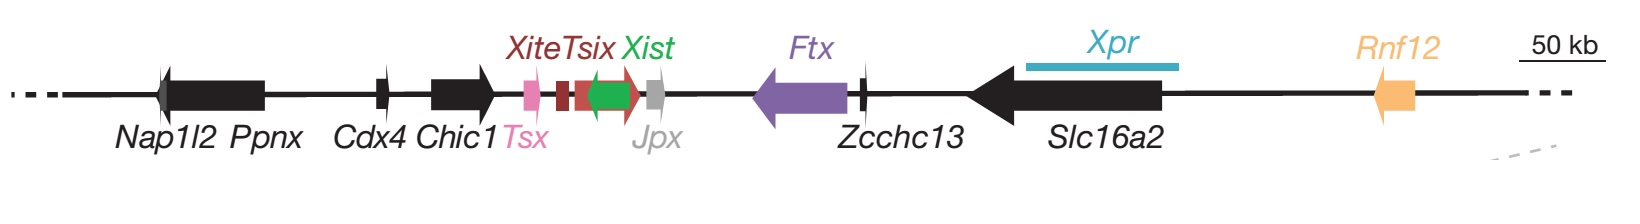
\includegraphics[scale=0.3]{geneSequencesTADDandE}
\caption{\scriptsize{The genes and non protein coding regions of TAD D and E. Image taken from from Nora et al.Nature. 2012 Apr 11;485(7398):381-5 \cite{nora2012spatial}}}
\label{figure_genesOfTadDandE}
\end{figure}

\section{A short review of Chromosome Capture methods}\label{section_chromosomeCaptureMethod}
The 5C method \cite{dostie2006chromosome} relies on the first steps of the seminal 3C method proposed by Dekker et al. 2002 \cite{dekker2002capturing}. 
From the \href{http://www.sciencemag.org/content/295/5558/1306/suppl/DC1}{supplementary material} of \cite{dekker2002capturing}. The steps of the 3C can be described as follows (see also Figure \ref{figure_3Cschematic}:

\begin{enumerate}
 \itemsep1pt \parsep0pt \parskip0pt 
\item Roughly $10^8$ intact nuclei are isolated
\item Nuclei are \href{http://en.wikipedia.org/wiki/Crosslinking_of_DNA}{cross-linked} by using $1\%$
\href{http://en.wikipedia.org/wiki/Formaldehyde}{formaldehyde}, or its relative paraformaldehyde, for 10 minutes, which induces protein-protein and DNA-protein cross-linking. The cross-link is made by formaldehyde in the guanine nucleotide, between DNA-bound proteins and the DNA. The \href{http://en.wikipedia.org/wiki/Lysine}{lysine} amino acid of the protein is connected through its $-NH_2$ group to the \href{http://en.wikipedia.org/wiki/Methylene_bridge}{Methylene bridge} ($-CH_2-$)

\begin{figure}[H]
\centering{
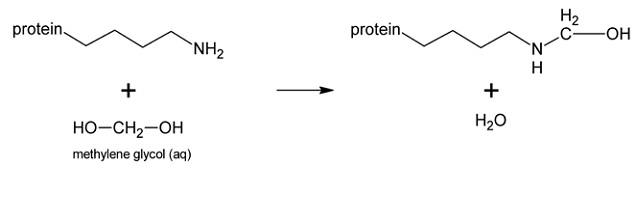
\includegraphics[scale=0.3]{crosslinkFormaldehydeProtein}
\caption{\scriptsize{The chemical bond between the $NH_2$ group of formaldehyde and the lysine $-NH_2$ group of the protein}}
\label{figure_crosslinkFormaldehydeProtein}
}
\end{figure}

Formaldehyde can be polymerized if alcohol is not added to it. Therefore, it is relevant to ask how the procedure in Nora et al \cite{nora2012spatial} was performed? 
\item Cross-linking distance is between $10-100nm$ \cite{dekker2013exploring}
\item All non cross-linked proteins are removed. It is important to note that the DNA is purified from non cross-linked proteins only \textit{after} the cross-links were made.
\item A site-specific restriction enzyme (\href{http://en.wikipedia.org/wiki/EcoRI}{EcoRI} or \href{http://en.wikipedia.org/wiki/HindIII}{HindIII}, which are 6bp cutters) is used to digest the cross-linked DNA for 1 hour. 
\item The restriction enzymes are inactivated using SDS and incubation for 20 minutes.
\item The reaction is 15 times diluted to favor relevant DNA-end ligation.
\item The free ends of the cleaved DNA are ligated (DNA is still cross-linked with proteins) for 45 minutes using \href{http://en.wikipedia.org/wiki/Ligase}{ligase}.
\item Reverse cross-linking by overnight incubation: the cross-links are destroyed, leaving segments of ligated DNA. The reverse cross-linking is done by incubation at $70^0$.
\item DNA is purified from non cross-linked proteins.
\item The products of the ligation are detected and quantified using PCR, by designing primers to specific ligation junctions. 
\item a control template is created by using the same restriction enzyme on non cross-linked DNA and ligation of DNA fragments without dilution
\end{enumerate}

\begin{figure}[H]
\centering{
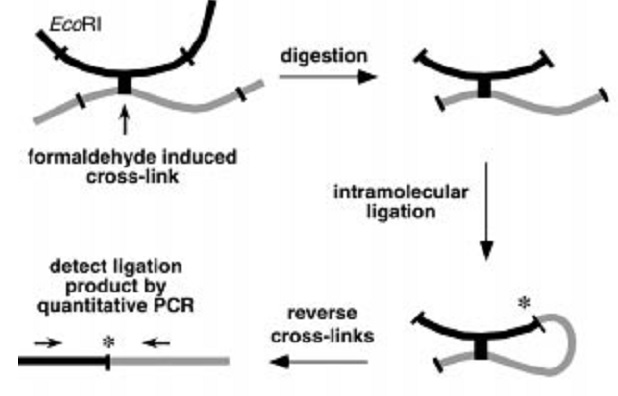
\includegraphics[scale = 0.4]{3Cschematic}
\caption{\scriptsize{A schematic representation of the 3C method. Image taken from Dekker et al. 2002 \cite{dekker2002capturing}}}
\label{figure_3Cschematic}
}
\end{figure}

\section{The Experimental Data}\label{section_theExperimentalData}
Two replicates of 5C experiments were conducted on the chromosome region encompassing the Xic region. The data was coarse-grained as explained in \ref{subsection_coarseGrainingOfEncounterData}, in accordance with the procedure by \cite{giorgetti2014predictive}\cite{nora2012spatial}.
The encounter data includes 14,508 pairwise encounters of genomic loci. Each genomic segments is defined by a start and end-bead index.

\section{Analysis of the experimental data}\label{section_AnalysisOfTheExperimentalData}

\subsection{Coarse-graining of the data}\label{subsection_coarseGrainingOfEncounterData}
The following paragraphs are an adapted version of the text in from Giorgetti et al. \cite{giorgetti2014predictive} supplementary material.

In the genomic region of the TAD D and E, 124 forward (FOR) and 126 reverse (REV) primers anneal to alternate HindIII restriction fragments of variable size. 
Since the average length of FOR and REV fragments in this region is 3078 bp, a 3000-bp beads was chosen, resulting in polymers of N=108 beads in the case of TAD D alone (chrX:100378306-100699670, total length 321,364 bp) and $N=307$ beads in the case of TAD D+E (total length 920,432 bp). Thirty five percent of restriction fragments were longer then 3000 bp and were mapped on multiple beads, while the remaining $65\%$ contributed, together with their nearest neighbor, to define the expected contacts of single beads.

The uneven sampling of the genomic region, provided by restriction fragments of different length, must be mapped onto the even sampling provided by equally spaced beads. This is performed as follows\cite{giorgetti2014predictive}:
\begin{enumerate}
 \itemsep1pt \parsep0pt \parskip0pt 
\item The $5$ end of the first bead in the chain is positioned at the 5’ end of the first restriction fragment in the region of interest 
\item Each restriction fragment in the region is assigned two indices $i$ and $j$ $(i,j=1…N)$ corresponding to the beads to which its 5’ and 3’ ends overlap.
\item 5C counts corresponding to each pair of restriction fragments are assigned to the corresponding pairs of indices (i,j) and (h,k), for example:
\item If two or more consecutive FOR or REV restriction fragments map to the same bead, their contributions are summed ($<10\%$ of all interactions).
\item 5C counts of two experimental replicates are averaged for each pair of restriction fragments and their standard deviation is taken as a measure of experimental uncertainty.
\end{enumerate}

\subsection{The encounter matrix}\label{subsection_theEncounterMatrix}
The data provided by Giorgetti et al.\cite{giorgetti2014predictive} contains the encounter frequency of beads (not segments!) constructed as explained in \ref{coarseGrainingOfEncounterData}. Sorting the encounter data into a 307 by 307 matrix we can visualize the pair-wise encounter frequencies. Reminder: beads are numbered sequentially from the 5-end to the 3-end of the polymer.


\subsection{From encounter frequency to encounter probability} \label{subsection_fromEncounterFrequencyToEncounterProbability}
We start by transforming the encounter frequency into encounter probability as follows. Each line of the encounter matrix is divided by the sum of all encounters of the line.

\subsection{Showing the TADs}\label{subsection_showingTheTADs}
TADs are seen by displaying the normalized encounter data, after removing closest beads data from the matrix of encounters. 
The normalization is done by taking each row $k$ of the encounter matrix, removing the data for the closest neighbors of bead $k$ and dividing by the sum of the row. A median filter of size 30 beads is then applied to the image (see methods in \cite{nora2012spatial}). 
 
\subsection{Symmetry of encounter frequency data}
We next examine whether the data can be regarded as symmetric in the sense of encounter probabilities for each bead. That is, whether bead $k$ has the same probability to meet its closest neighbors from the right and left in the linear chain, or not.  

The symmetry of encounter frequency data is shown by measuring the left and right encounter frequencies of each one of the beads comprising the chain.
The left and right encounter data are defined in terms of bead index, where for the bead $j$ the left encounter frequencies are defined as a vector of length $j-1$ with the encounter data of bead $j$ with $1,..,j-1$, and $j+1,..,N$ for the right encounter frequencies. 

For bead index $j=1,...,N$ we have different number of beads on the left and right. For comparison, we need to match the number of beads from the left and right for each bead. The number of beads on the left and right of bead $j$ is then taken to be $n_j=min(j-1,N-j+1)$. 
Let $L_j$ be the left encounter data, $R_j$ be the right encounter data vectors of lengths $n_j$
\begin{equation*}
L_j=\left[e(j-1),e(j-2),...e(j-n_j)\right] 
\end{equation*}
and 
\begin{equation*}
R_j=\left[e(j+1), e(j+2),...,e(j+n_j)\right]
\end{equation*}
where $e(k)$ is the encounter frequency of the $k^{th}$ closest bead to bead $j$. Note the reverse order of $L_j$.

We normalize each vector by dividing it by the sum of its encounters
\begin{equation*}
\hat{L_j} =\left[e(j-1),e(j-2),...,e(j-n_j)\right]/\sum_{k=j-n_j}^{j-1}e(k)
\end{equation*}
and similarly for $\hat{R}_j$.

To test the difference between left and right frequencies, we calculate the mean difference by 
\begin{equation*}
d_j=\frac{1}{n_j}\sum_{k=1}^{n_j} \left(\hat{L_j}(k)-\hat{R_j}(k)\right)
\end{equation*}

The Figure \ref{figure_resultsOfFrequencyDifference} below shows the results of plotting the mean difference for the two replicates of the 5C data 

\begin{figure}[H]
\includegraphics*[scale=0.3]{symmetryOfEncountersRep1.jpg}
\includegraphics*[scale=0.3]{symmetryOfEncountersRep2}
\includegraphics*[scale=0.3]{symmetryOfEncountersAverage}
\caption{\scriptsize{ The mean difference (y axes) between left and right encounter frequencies for each bead number (x axes) is shown for Rep1 (top left) Rep2 (top right) and average (bottom)}}
\label{figure_resultsOfFrequencyDifference}
\end{figure}  

The red lines in the Figure \ref{figure_resultsOfFrequencyDifference} signify the mean of the difference data. For the three figures it is of the order $10^{-18}$. When points are missing, it means that the segment (restriction segment) occupies more than one bead, therefore the encounter data is zero there. 

We can therefore treat the right and left data in the same manner and 'fold' the encounter data such that from now on we test the encounter data by bead distance. We will refer to the one-sided encounter as the encounter data from now on. 

\subsection{Peaks of the encounter data}\label{subsection_peaksOfTheEncounterData}
For some beads the encounter data shows peaks at some distance from the origin (Figure \ref{figure_peaksOfTheEncounterProbabiltity307Beads}). 
These peaks represent a frequent encounter with a distal part of the chain. The list of bead numbers and the frequent encounter they have with the distal chain parts (represented by bead numbers) is summarized in Table \ref{table_peaksOfTheEncounterDataOneSided}

%TODO: the figure below should be replaced
\begin{figure}[H]
\includegraphics*[scale=0.2]{EncounterFrequenciesByDistanceRep1}
\caption{\scriptsize{The encounter probability of each bead (Y axis) as a function of bead distance (X axis). The dashed red rectangles shows places of prominent non-nearest neighbors encounters}}
\label{figure_peaksOfTheEncounterProbabiltity307Beads}
\end{figure}

% One Sided prominant encounters
\begin{table}[H]\label{table_peaksOfTheEncounterDataOneSided}
\begin{tabular}{l l l}
bead numbers & encountered beads & TAD\\
\hline
23-26   & 280-290 & $D\leftrightarrow E$\\
49-53   & 148-155 & $D\leftrightarrow E$\\
56-59   & 80-90   & $D\leftrightarrow D$\\
115-117 & 165-170 & $E\leftrightarrow E$\\
161-162 & 187 190 & $E\leftrightarrow E$\\
182-184 & 260-264 & $E\leftrightarrow E$\\
185-186 & 253-255 & $E\leftrightarrow E$\\
234-236 & 184-189 & $E\leftrightarrow E$\\
234-236 & 4-11    & $E\leftrightarrow D$\\
243     & 88      & $E\leftrightarrow D$\\
264     & 89-90   & $E\leftrightarrow D$\\
274-277 & 113-120 & $E\leftrightarrow D(?)$
\end{tabular}
\end{table}

% two sided prominant encounters 
\begin{table}[H]\label{table_peaksOfTheEncounterDataTwoSided}
\begin{tabular}{l l l l}
bead numbers & encountered beads & TAD & rep\\
\hline
1       & 86      & $D\leftrightarrow D$& 1 \\
6       & 81      & $D\leftrightarrow D$& 1 \\
6       & 227-229 & $D\leftrightarrow E$& 1 \\
6       & 243     & $D\leftrightarrow E$& 1 \\
7       & 81      & $D\leftrightarrow D$& 1 \\
7       & 226-229 & $D\leftrightarrow E$& 1 \\
7       & 247     & $D\leftrightarrow E$& 1 \\
10      & 77      & $D\leftrightarrow D$& 1 \\
10      & 77      & $D\leftrightarrow D$& 1 \\
23      & 293     & $D\leftrightarrow E$& 1 \\
24      & 264     & $D\leftrightarrow E$& 1 \\
25      & 285     & $D\leftrightarrow E$& 1 \\
26      & 285     & $D\leftrightarrow E$& 1 \\
26      & 86      & $D\leftrightarrow D$& 1 \\
26      & 59-74   & $D\leftrightarrow D$& 1 \\
49-53   & 150     & $D\leftrightarrow E$& 1 \\
64-66   & 287     & $D\leftrightarrow E$& 1 \\
65-66   & 34      & $D\leftrightarrow D$& 1 \\ 
64,67-69& 26      & $D\leftrightarrow D$& 1 \\       
71      & 24      & $D\leftrightarrow D$& 1 \\
72-75   & 26      & $D\leftrightarrow D$& 1 \\

\end{tabular}
\end{table}

The question arises as to whether these frequent encounter represent a loop in the polymer chain or is it the results of the 3D structure of the folded polymer? Since the 5C data is essentially taken over millions of cells it remains to show that these encounters (or loops) are indeed conserved elements of the Xic region in cells and not a result of averaging in the population level.

\subsection{Fitting the encounter data}\label{subsection_fittingTheEncounterData}
In this and subsequent sections we work with the first replicate of the data.

To examine the behavior of the polymer as a whole, we fit for each bead's encounter data 
a function of the form 
\begin{equation}\label{equation_fitModel}
e_j(d)= \frac{1}{\sum_{i=1}^{N_j}d_i^{-\beta}}d^{-\beta}
\end{equation}
$e_j$ is the normalized encounter frequency of bead $j$, $d$ is the distance in bead units , and $\beta$ is a parameter to be determined by the fitting process. 

The fitted exponent ($\beta$) value obtained by minimizing the error in the model \ref{equation_fitModel} are shown in Figure \ref{figure_fittedExpExperimentalData307Beads}
\begin{figure}[H]
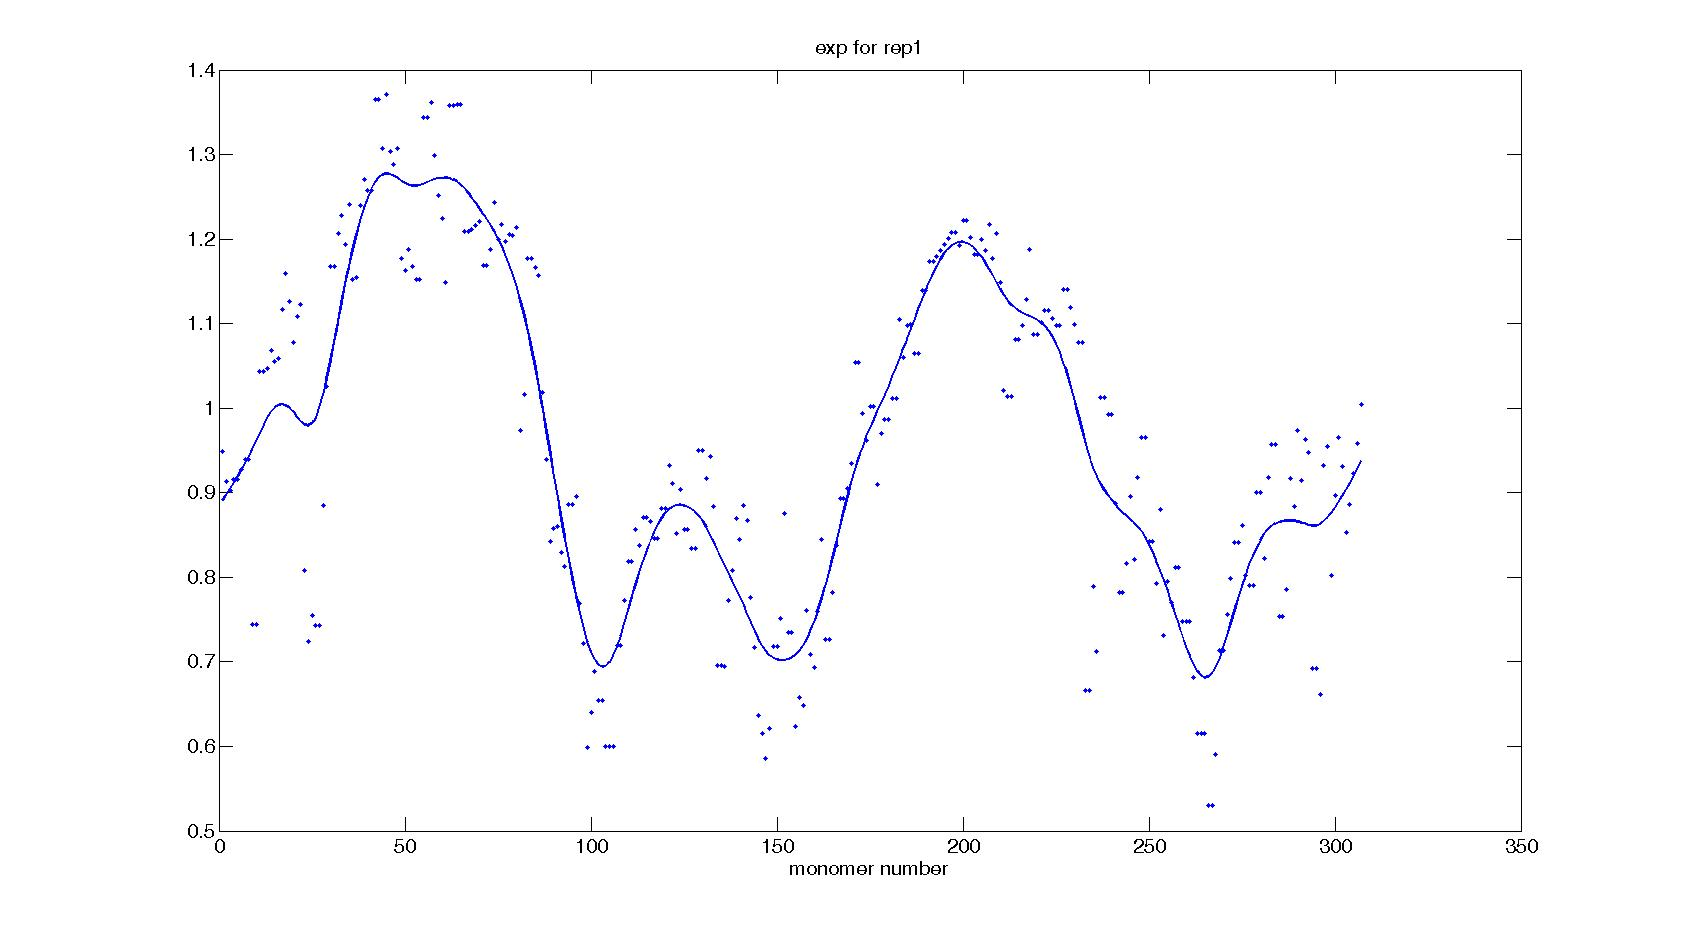
\includegraphics[scale=0.15]{fittedExpValuesWithSplineRep1}
\caption{\scriptsize{The fitted $\beta$ value for each bead 1 to 307. The continuous curve represents a smoothing of the fitted exponent values using a smoothing spline with tolerance of 2 (see Matlab documentation on \href{http://www.mathworks.fr/fr/help/curvefit/spaps.html}{spaps} function)}}
\label{figure_fittedExpExperimentalData307Beads}
\end{figure}

In Figure \ref{figure_fittedExpExperimentalData307Beads}, we see that the fitted exponent curve is somewhat tri-modal. With one peak located in roughly at bead 54, one at 125, and the left most at 200. The first and the last places correspond the mid points of the two TADs of the encounter. 


\subsection{Heterogeneity of the parameters over the beads}
The question arises as to whether the beads behave in a similar manner in terms of parameter values (i.e obey the same model rules), and if not, would it be possible, just by assuming a model, to identify beads belonging to the same group, and elucidate the similarity or difference between groups of beads. 
We start by looking at adjacent beads properties according to the resulting parameter fitted.
To simultaneously see the heterogeneity of the fitted parameters over all beads, we calculate the pairwise difference between parameters of the beads. 
the resulting matrices take the shape

\begin{figure}[H]
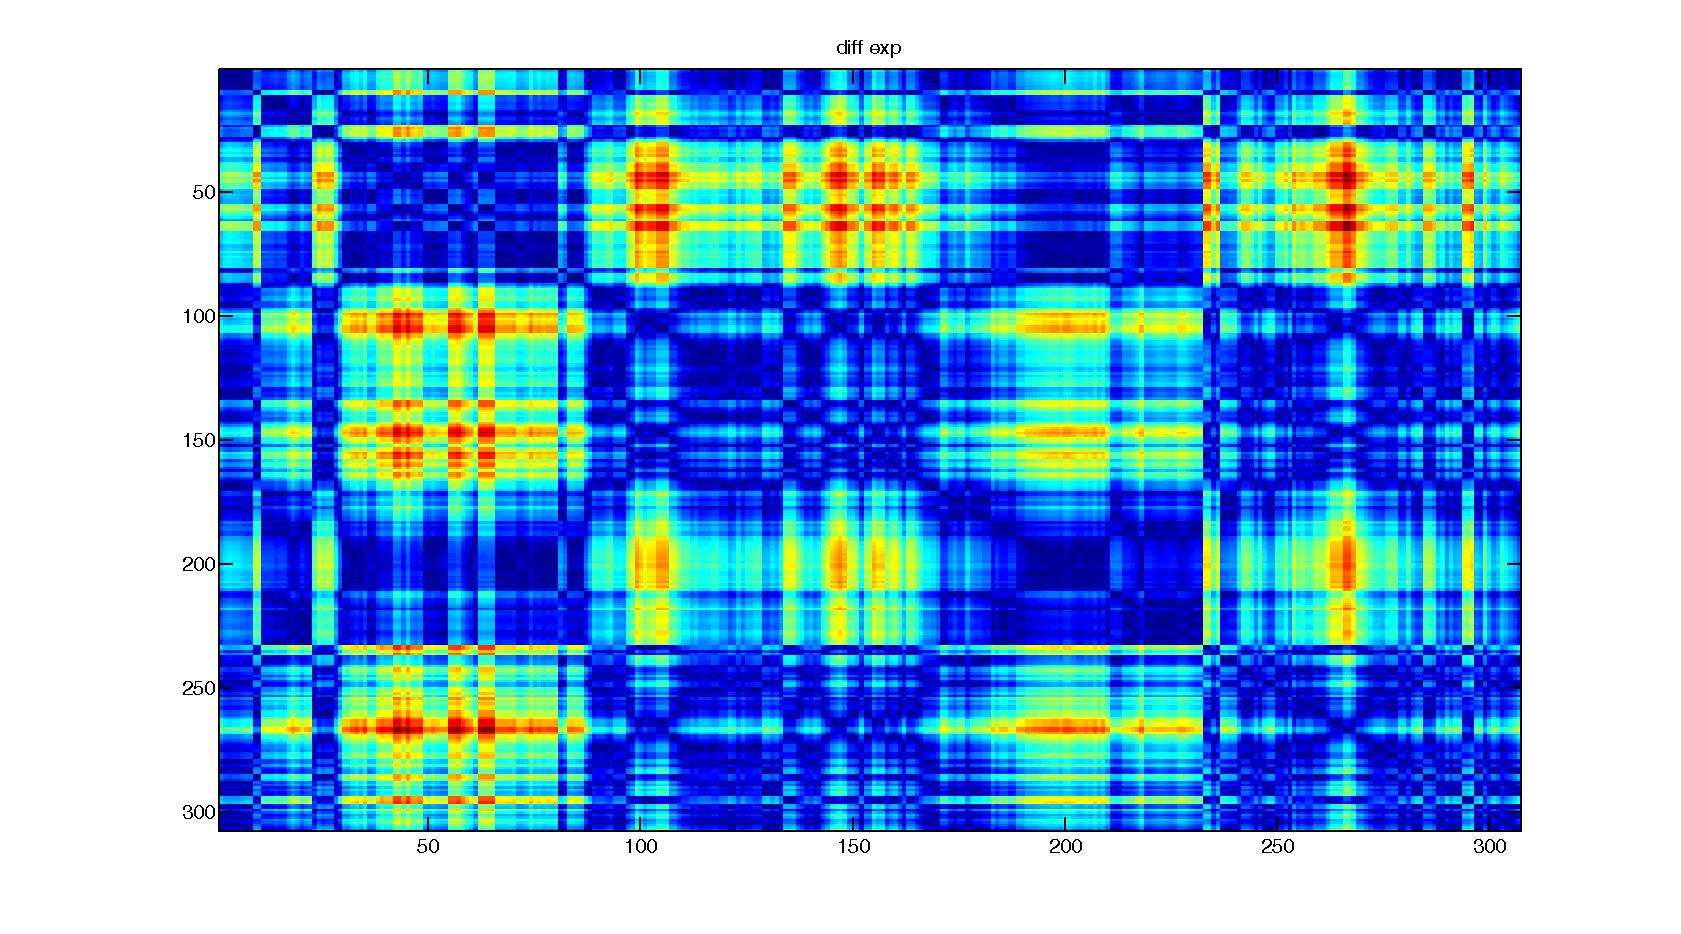
\includegraphics[scale=0.12]{diffFittedExpRep1}
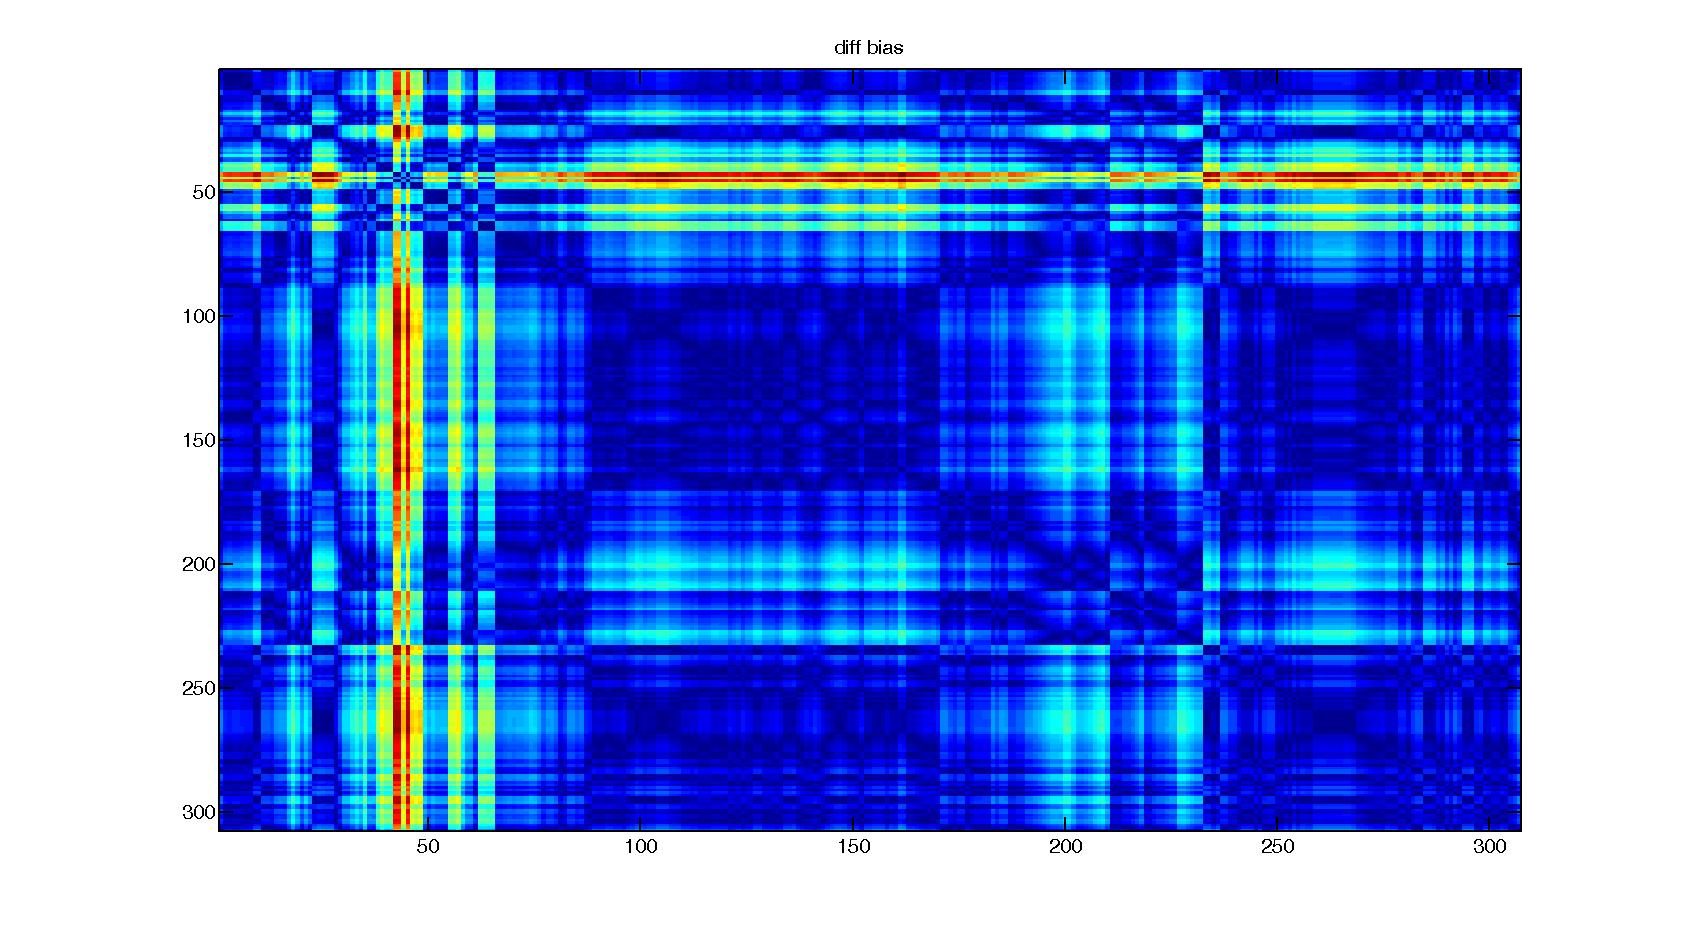
\includegraphics[scale=0.12]{diffFittedBiasRep1}
\includegraphics[scale=0.12]{normDiffFittedExpfittedBiasRep1}
\caption{\scriptsize{The norm of the difference between the fitted parameters from model \ref{equation_fitModel} in a pairwise manner. the columns and rows represent bead numbers. The pairwise exponent difference norm (top), the pairwise difference norm for bias (middle); the norm of the two difference matrices (bottom)}}
\label{figure_diffFittedParametersRep1}
\end{figure}

It is now also apparent from Figure \ref{figure_diffFittedParametersRep1} that beads 35-50 have different bias values then expected. To find beads for which the exponent values agree but the bias values do not, we search for a threshold for the difference of exponents and bias below which it could be said that values are similar. 
For this end, we can consider the data as having 'low' and 'high' difference values. 
We search for a values $v_{exp}$ and $v_{bias}$ for which the 'within' group variance is low and the 'between' group variance is the highest. 
Such approach leads naturally to employ the \href{http://en.wikipedia.org/wiki/Otsu's_method}{Otsu} method. Using this method on the matrix, the value of $v_{exp},v_{bias}$ are found to be 

\begin{equation*}
v_{exp}= 0.262
\end{equation*}
\begin{equation*}
v_{bias}=0.18
\end{equation*}

\chapter{Simulations}
\section{The Simulation Framework}
We have constructed a computational stochastic simulation framework, which allows us to examine the behavior of the polymer chain in various configurations.
We use the \href{http://en.wikipedia.org/wiki/Rouse_model}{Rouse model} to mathematically describe the polymer chain as a series of beads connected by harmonic springs (see figure \ref{figure_exampleOfChains}). The stochastic differential equation describing the dynamics of bead $n$ in a chain of $N$ beads is 
\begin{equation*}
\dot{r_n} = -D\nabla_{r_n}\phi_{Rouse}+\sqrt{2D}\dot{w_n}
\end{equation*}
with the potential 
\begin{equation*}
\phi_{Rouse}=\frac{\kappa}{2}\sum_{n=1}^N \left(r_n-r_{n-1}\right)^2
\end{equation*}
which in the linear chain case gives rise to the set of equations
\begin{equation*}
\dot{r_n}= -\frac{d\kappa D}{b^2}\left(2r_n-r_{n+1}-r_{n-1}\right)+\sqrt{2D}\dot{w_n}
\end{equation*}
for the inner beads, and 
\begin{eqnarray*}
\dot{r_1} &=& -\frac{d\kappa D}{b^2}\left(r_1-r_{2}\right)+\sqrt{2D}\dot{w_1}\\
\dot{r_N} &=& -\frac{d\kappa D}{b^2}\left(r_N-r_{N-1}\right)+\sqrt{2D}\dot{w_N}
\end{eqnarray*} 
for the end beads. Where $r_n$ are the coordinates of the $n^{th}$ bead, $d$ is the dimension, $\kappa$ is the spring constant, $D$ is the diffusion constant, $b$ is the standard-deviation of the distance between adjacent beads, and $w$ is N-dimensional white Gaussian noise with mean 0 and variance 1 in each component. 


The flexibility of our framework enables us to simulate a single or an ensemble of chains in open space or in 3 types of domains: a sphere, a cylinder, and between two infinite plates. As an extension to the classical Rouse model, we can also simulate the chain with variable minimal distance, $l_0>0$, between adjacent beads. Hence, we modify the Rouse potential to read
\begin{equation*}
\phi_{Rouse}=-\frac{\kappa}{2}\sum_{n=1}^N\left((\|r_n-r_{n-1}\|-l_0)^2\right)
\end{equation*}
and simulate the coupled (coordinate-wise) system of equations it yields.

In addition, non-adjacent beads can be fixed to form stable loops throughout the simulation (see Figure \ref{figure_exampleOfChains} left panel). In the course of simulation (such as in subsection \ref{RandomFixedLoops}), we can randomize the location of these fixed loops, a model we name \textit{random fixed loop model}. We extend this idea to allow the formation and dissociation of loops in time, a model termed dynamic loop model. In this model only when the affine beads are located within some minimal distance $\epsilon$ to one another they form a loop with association rate $\lambda$ per unit of time. Looped affine beads can dissociate with dissociation rate $1-\lambda$.

At the end of simulations, an analysis is performed to calculate the encounter probability between beads of the chain, and a report is generated.  

We consider that two beads $R_i$ and $R_j$ had encountered if
\begin{equation*}
 dist_{ij}=\|r_i-r_j\|\leq \epsilon
\end{equation*}
with $0<\epsilon <b$. The theoretical encounter probability in a linear Rouse chain is given by 
\begin{equation}
Pr(dist_{ij}<\epsilon)= \alpha |i-j|^{-1.5}
\end{equation}
with $\alpha>0$. 

At the end of simulations we extract the encounter histogram of beads and fit it with a function of the form 
\begin{equation*}
Pr(dist_{ij}\leq \epsilon)=\alpha_{ij}|i-j|^{-\beta}
\end{equation*}
for each pair of beads in the chain. 
\begin{figure}[H]
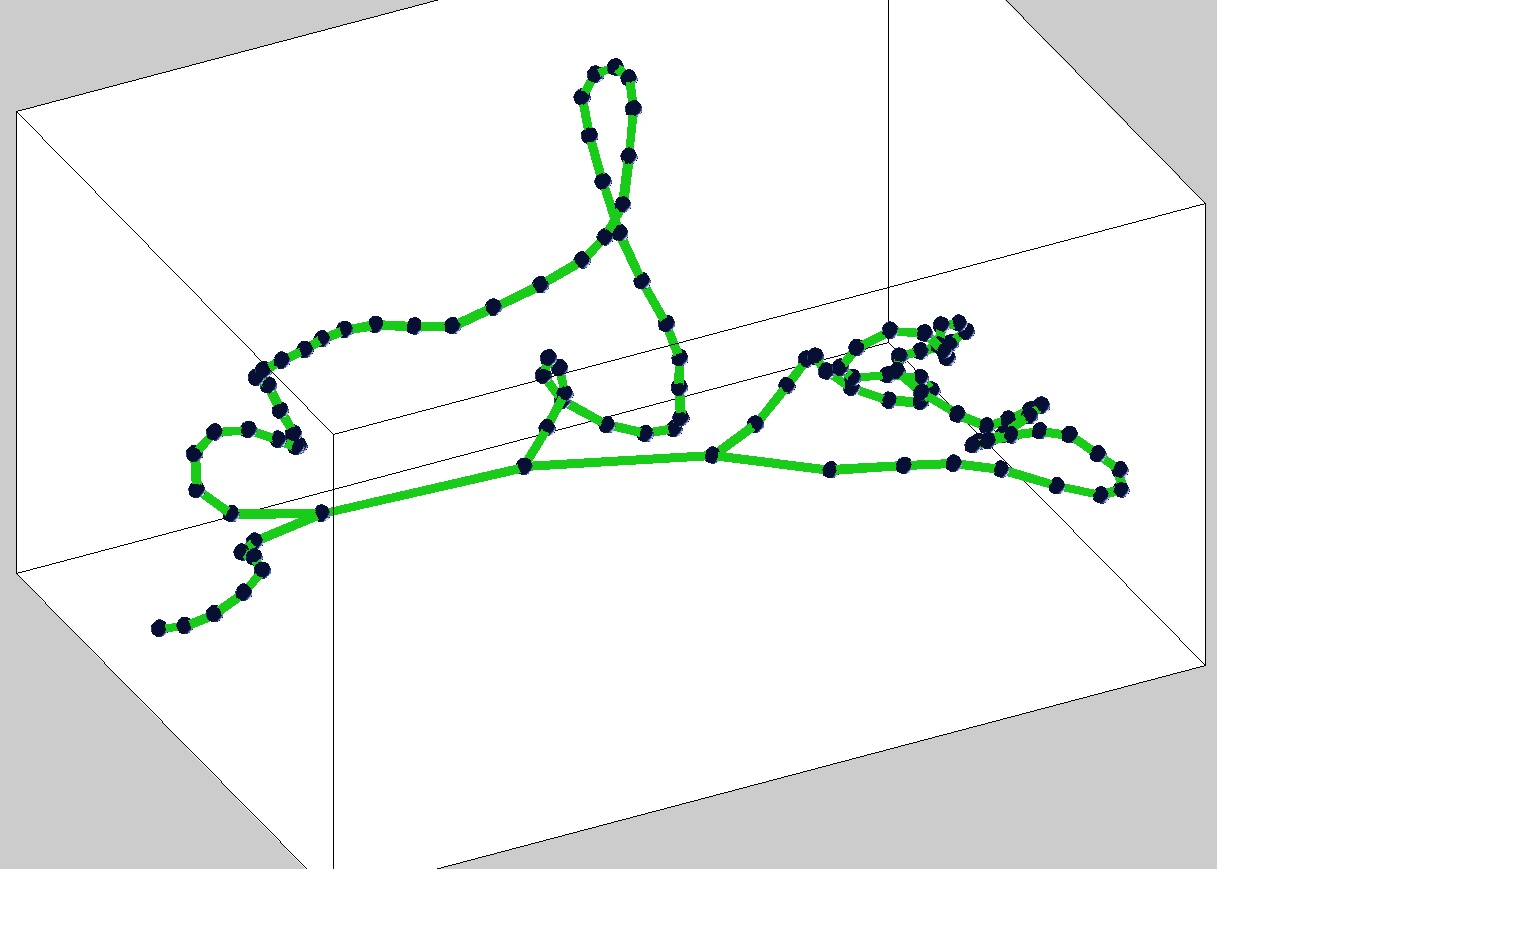
\includegraphics[scale=0.2]{chainExample108BeadsWith2Loops}
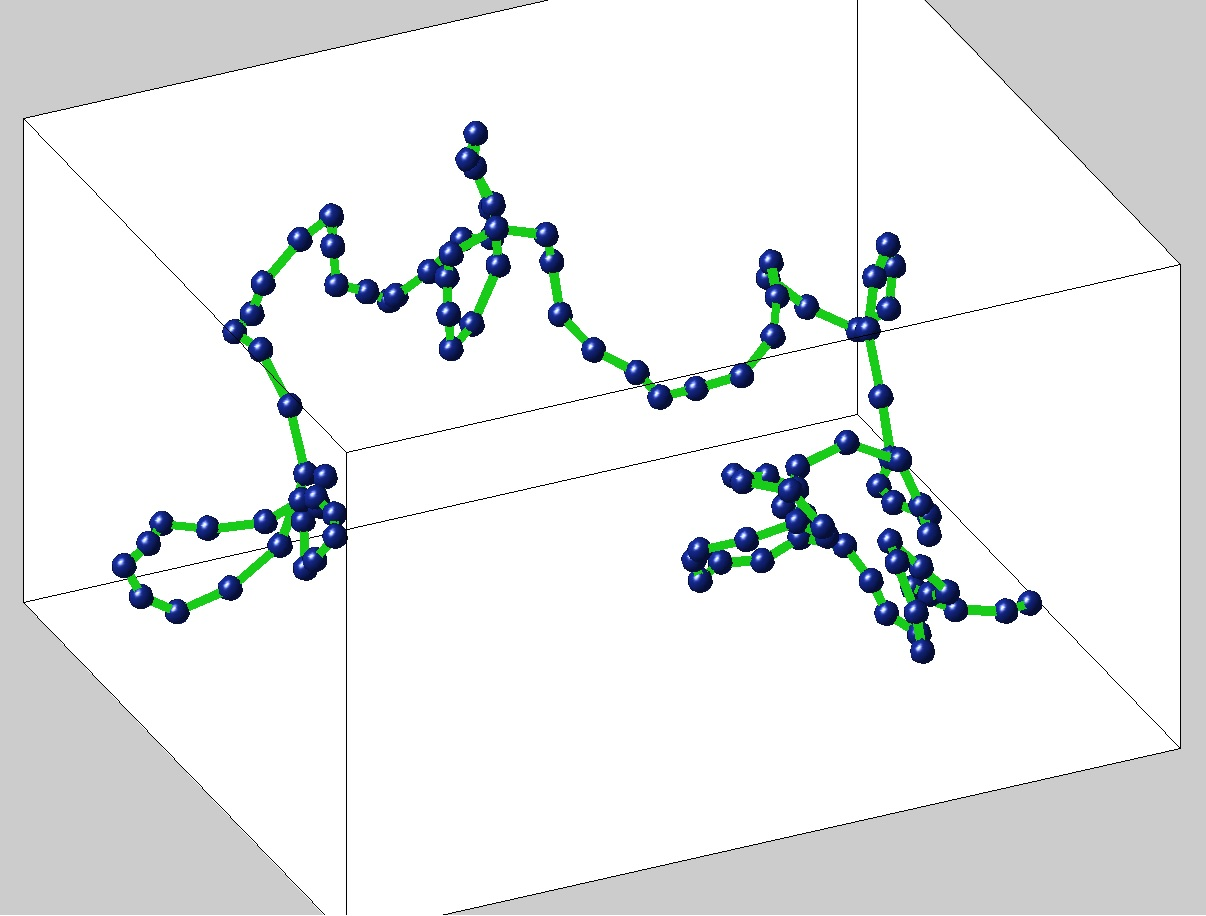
\includegraphics[scale=0.2]{chainExample108Beads}
\caption{\scriptsize{Two examples of the beads-springs model. A linear chain model (Right) and a chain with internal 2 loops (Left)}}
\label{figure_exampleOfChains}
\end{figure}


\section{Initial simulation settings}\label{section_initialSimulationSettings}
For the subsequent simulations, unless stated otherwise, we determine the simulation time step,$\Delta t$ and the simulation time as follows. 
the simulation step $\Delta t$  was determined such that it will prevent simulation 'blow-ups'
\begin{equation*}
 \Delta t = \frac{b^2}{12D}
\end{equation*}
Which is the values that stabilizes the numerical solution to the ode with no noise. when noise is present, this values can be increased.

The \textit{chain relaxation time} is given by 
\begin{equation*}
\tau_p = \frac{b^2\Delta t}{12d^2\sin^2(\frac{p\pi}{2N})}
\end{equation*}
where $p$ is the mode number. For simulations we use the relaxation time of the slowest mode $p=1$.

\section{Verification of the validity of simulation framework}
Here we make sure that the output simulation framework obeys the expected behavior of the Rouse polymer. 
A polymer of 64 beads, with no cross-linking is simulated for $40,000$ steps, the STD of link length was set to $b=0.1$. The result is presented in Figure \ref{figure_vereficationOfModelDistanceMatrix64Beads}

\begin{figure}[H]
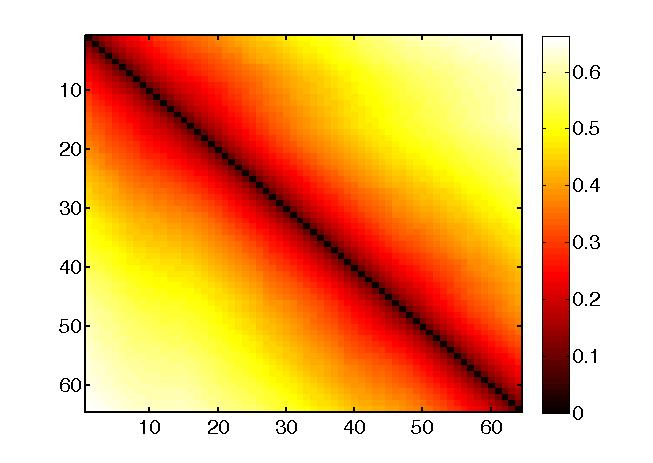
\includegraphics[scale=0.3]{distanceMatrix64Beads}
\caption{\scriptsize{The mean bead distance matrix after $50,000$ steps of the Rouse model}}
\label{figure_vereficationOfModelDistanceMatrix64Beads}
\end{figure}

For an easier comparison of the simulation output with theoretical results, we work from now on with the Root-Mean-Square (RMS) distance between beads. 

To see the expected increase in distance, we plot the cross-section of the RMS distance of the first bead to beads $2,3,..,64$. The distribution of distances between any two beads $n$ and $m$ of the Rouse polymer, have the following distribution
\begin{equation}
\Phi(R_n-R_m,n-m)=\left[\frac{3}{2\pi b^2|n-m|} \right]^{3/2}\exp{\left[-\frac{3(R_n-R_m)^2}{2|n-m|b^2} \right]}
\end{equation}

Where, $R_n$ is the vector of coordinates of bead $n$. The equation above is the consequence of the fact that the sum of normally distributed random variables is again a normally distributed random variable. In addition, it can be shown that 

\begin{equation}\label{RmsDistance}
<(R_n-R_m)^2>=|n-m|b^2
\end{equation}

Using the result above we compare the RMS distance between bead $1$ and beads $2,3,..,64$ with the function $|n-m|b^2$, appearing in equation \ref{RmsDistance}, with $b=0.1$. As can be seen from Figure \ref{figure_rmsDistanceBead1ToBeads2To64AndTheoreticalResults}, there is an excellent agreement between the output of the simulations and the theoretical results.

\begin{figure}[H]
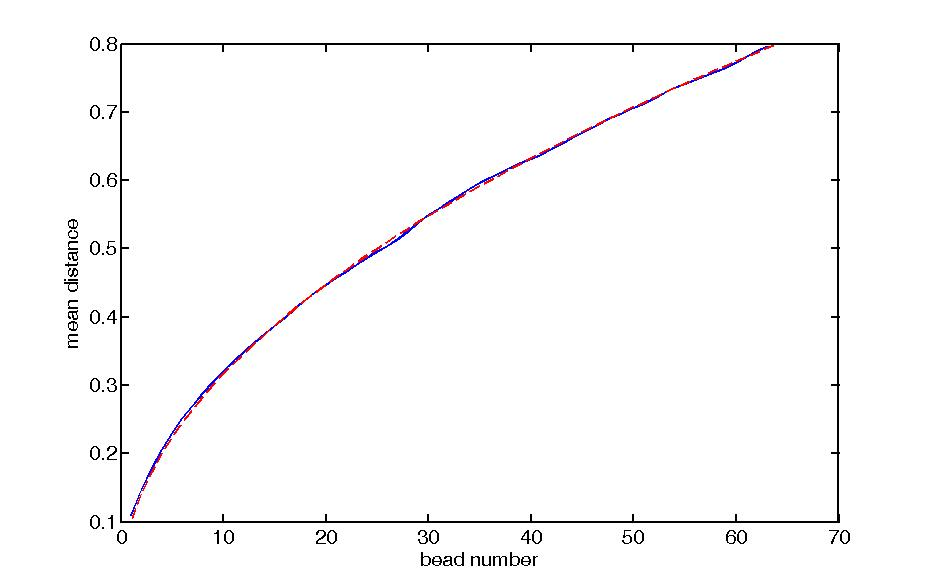
\includegraphics[scale=0.3]{rmsDistanceBead1ToBeads2To64AndTheoreticalResults}
\caption{\scriptsize{The RMS distance of bead 1 to all other 63 beads is plotted (blue curve) vs. the theoretical result (dashed red curve) $dist(1,n)=nb^2$. As can be seen, there is an excellent agreement between the curves, indicating that the simulation framework operates as expected}}
\label{figure_rmsDistanceBead1ToBeads2To64AndTheoreticalResults}
\end{figure}

The RMS distance between adjacent bead was found to be 0.105, in agreement with  the bond length $b=0.1$. The mean square end-to-end distance was found to be 0.6319, in agreement with the expected 0.64. Overall we can conclude that the system operates as expected.

\subsection{The encounter frequency}
According to the theory, the encounter frequency of a bead $m$ in a Rouse chain as a function of the distance of beads from it on the linear chain, should be proportional to $1/|m-n|$, where $n\ne m$ is the distance in bead units. To see that the simulation framework obeys this rule, the encounter frequency matrix was calculated. The encounter distance was set to $0.1$, the matrix is presented in Figure \ref{figure_encounterMatrix64Beads}. To see the decay of the encounter matrix, we  plot the normalized encounter events of bead 1, and present the fit of the function
\begin{equation}
y = ax^{-b}
\end{equation}
The encounter data was normalized prior to fitting by dividing it by the sum of encounter of bead 1. The parameters fitted were found to be $a=0.2436$ and $b=1.036$, in agreement with the expected $e(1)\propto 1/n$

\begin{figure}[H]
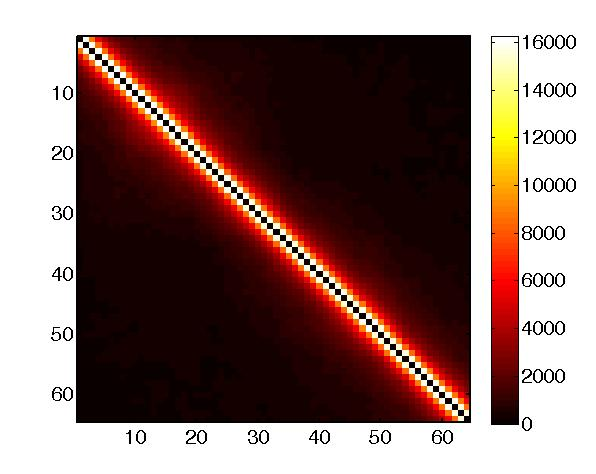
\includegraphics[scale=0.3]{encounterMatrix64Beads}
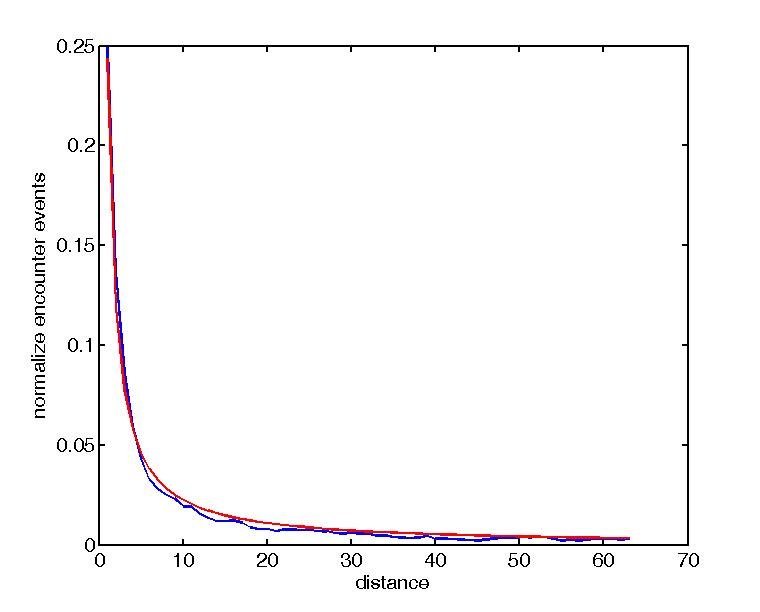
\includegraphics[scale=0.3]{encounterFrequencyBead1WithFit}
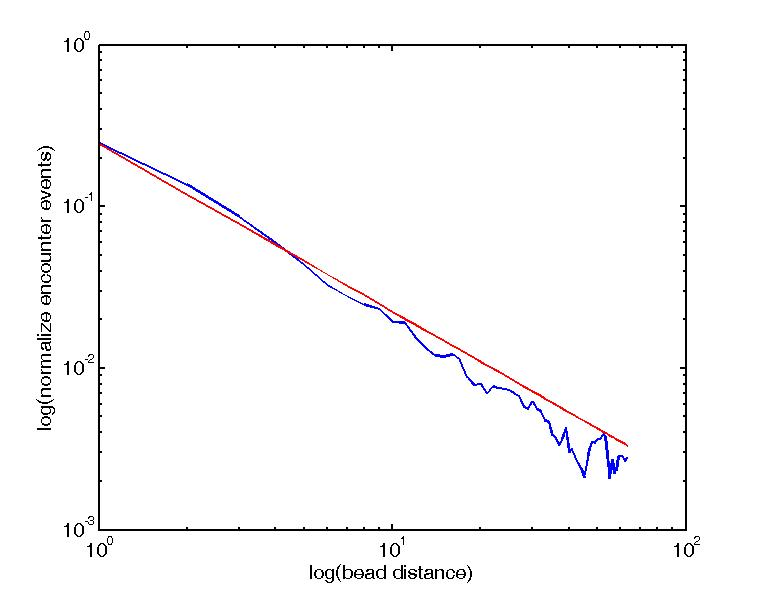
\includegraphics[scale=0.3]{encounterFrequencyBead1WithFitLogScale}
\caption{\scriptsize{The encounter frequency and verification of theoretical results. The encounter matrix (top left) for a 64 beads Rouse chain. The decay of the rows of the encounter matrix is presented for the first bead (top right) for which we have the most number of beads (blue line) and a fit to the encounter curve (red line). the encounter frequency of bead 1 in a log-log scale (bottom left, blue curve) and a fit according to the theory (red line).}}
\label{figure_encounterMatrix64Beads}
\end{figure}

\section{A polymer with a single cross-link}\label{section_aPolymerwithASingleCrossLink}
Next, we calculate the distance matrix for a 64 bead polymer for which bead 24 and 44 are cross-linked, creating a loop of size 20 [beads]. 
The simulation is run from relaxation time, a total of $50,000$ steps. The relaxation time is determined according to the formula
\begin{equation}
\tau_p = \frac{b^2\Delta t}{12d^2\sin^2(\frac{p\pi}{2N})}
\end{equation}
For  $\Delta t=10^{-4}$, $p=1$, $d=\sqrt{2D\Delta t}$, $N = 64$, we get 
\begin{equation}
\tau_1 = 57.68 
\end{equation}
minutes, which is the relaxation time of the first Rouse mode derived from the cross-correlation function. 

\begin{figure}[H]
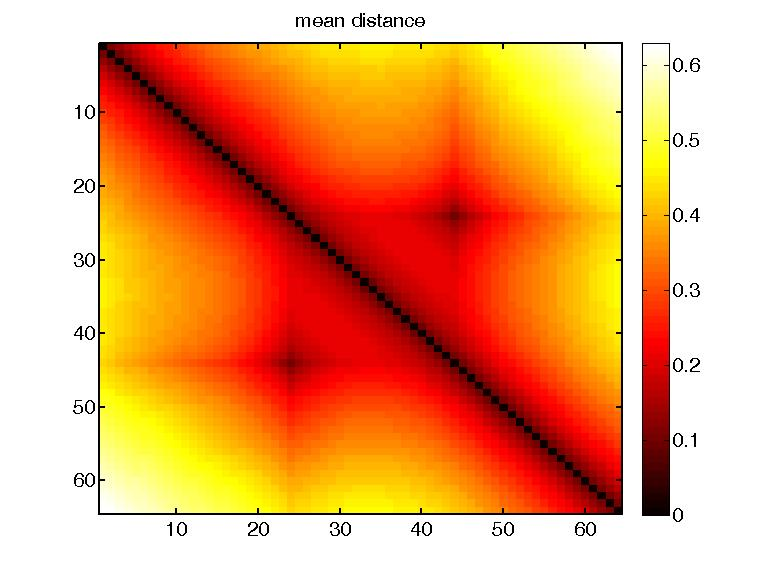
\includegraphics[scale=0.3]{distanceMatrix64BeadsConnect24And44}
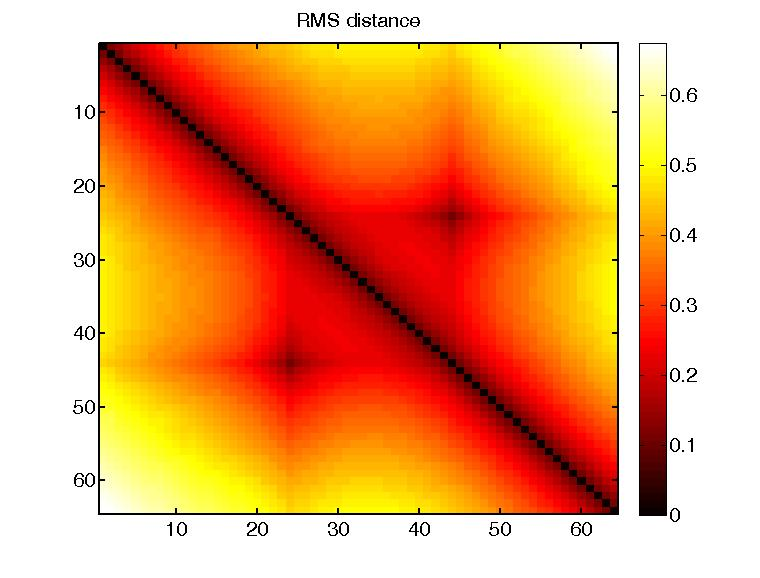
\includegraphics[scale=0.3]{rmsMatrix64BeadsConnect24And44}
\caption{\scriptsize{mean Distance matrix (left) and RMS distance matrix (right) over 50,000 steps of the simulation. Beads 24 and 44 are connected in a polymer of length 64 beads. As expected,the two matrices display similar qualitative behavior but with slightly different values}}
\label{figure_distanceMatrix64BeadsConnect24And44}
\end{figure}

To see the decay of bead distance, we plot the cross-sections of the bead-distance matrix presented in Figure \ref{figure_distanceMatrix64BeadsConnect24And44} at the rows 24 and 44. It 
\begin{figure}[H]
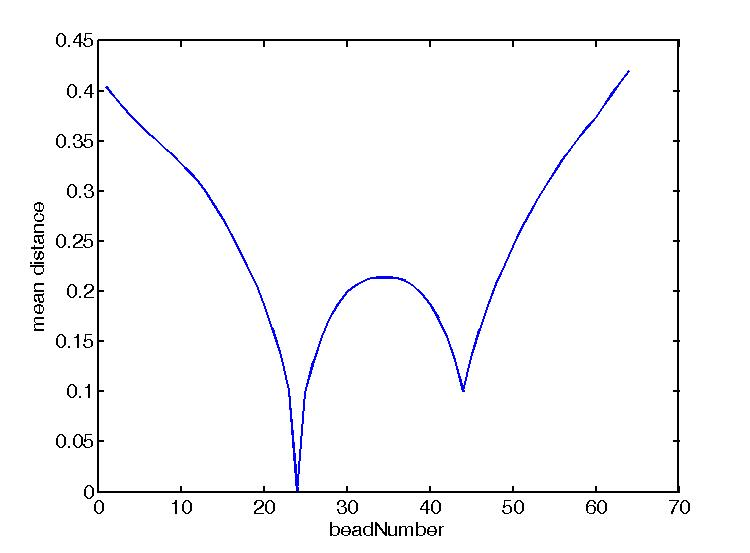
\includegraphics[scale=0.3]{crossectionAtRow24DistanceMatrix64BeadsConnect24And44}
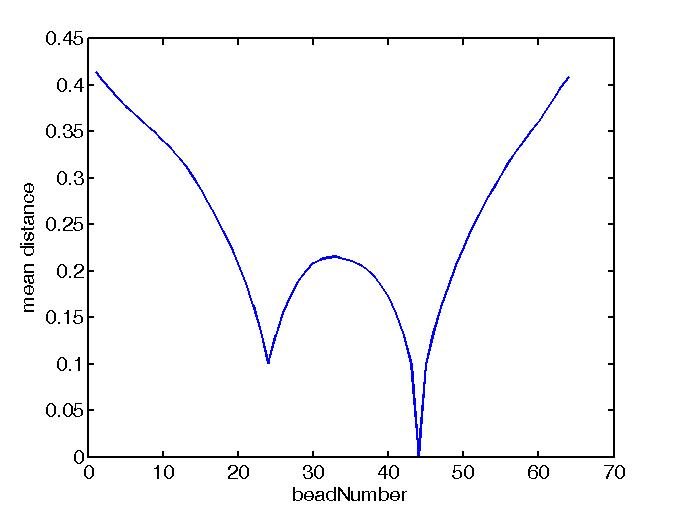
\includegraphics[scale=0.32]{crossectionAtRow44DistanceMatrix64BeadsConnect24And44}
\caption{\scriptsize{The cross section of the mean bead distance matrix presented in Figure \ref{figure_distanceMatrix64BeadsConnect24And44} for bead 24 (left) and bead 44 (right). The height at point 44 (left panel) and point 24 (right panel) is the bond length $b=0.1$ as expected.}}
\label{figure_crossectionAtRow24DistanceMatrix64BeadsConnect24And44}
\end{figure}

\subsection{Increasing the encounter distance}
Next we examined whether changing the encounter length in the cross-linked chain can explain the appearance of TADs. The encounter frequency between any two beads of the chain is shown in Figure \ref{figure_encounterFreq64BeadsConnect24And44VaryEncounterLength}. The encounter length varied between half and twice of the connector length (0.1).

\begin{figure}[H]
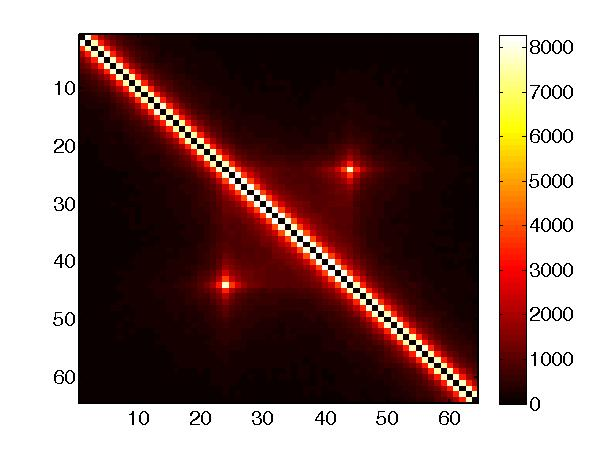
\includegraphics[scale=0.2]{encounterFrequency64BeadsConnect24And44EncounterDist0_05}
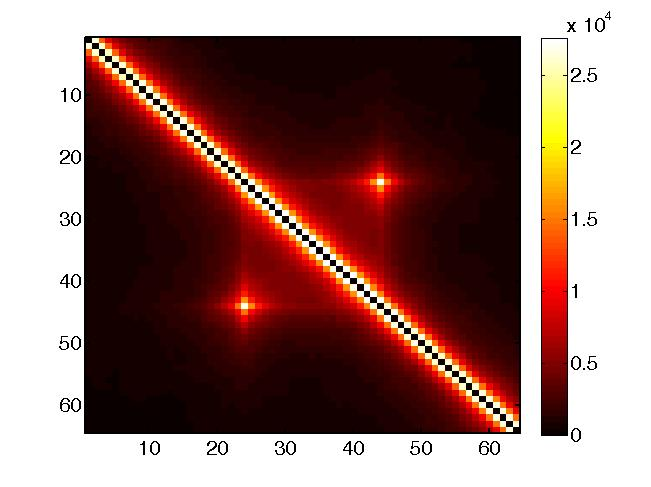
\includegraphics[scale=0.19]{encounterFrequency64BeadsConnect24And44EncounterDist0_1}
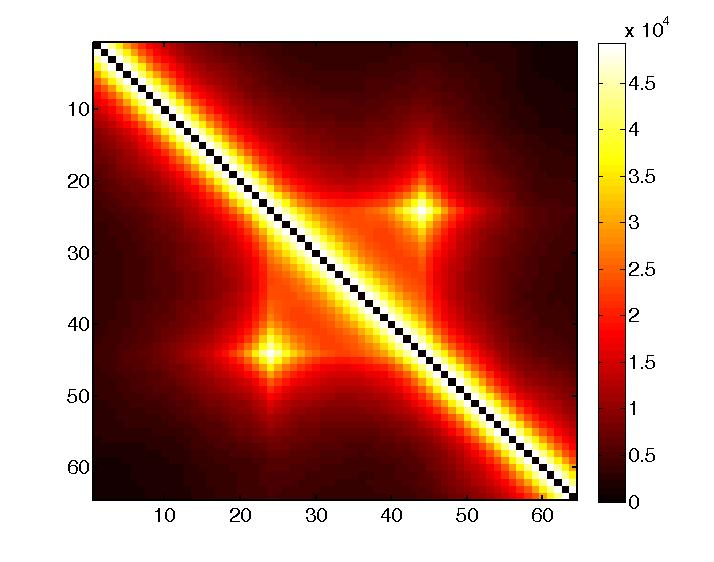
\includegraphics[scale=0.17]{encounterFrequency64BeadsConnect24And44EncounterDist0_2}
\caption{\scriptsize{Encounter frequency matrices of a Rouse polymer with 64 beads with bead 24 and 44 connected by harmonic potential when varying the encounter distance from 0.05 (left), 0.1 (middle), and 0.2 (right). The bond length was set to $b=0.1$, the encounter distance was set to 0.1. Simulation ran over 50,000 steps of $10^{-4}$ seconds. Each pixel represent bead pair $(i,j)$ of the polymer.}}
\label{figure_encounterFreq64BeadsConnect24And44VaryEncounterLength}
\end{figure}

The encounter histogram of bead 24 is displayed in Figure \ref{figure_encounterHistBead24connect24And44EncounterDist0_1}.
\begin{figure}[H]
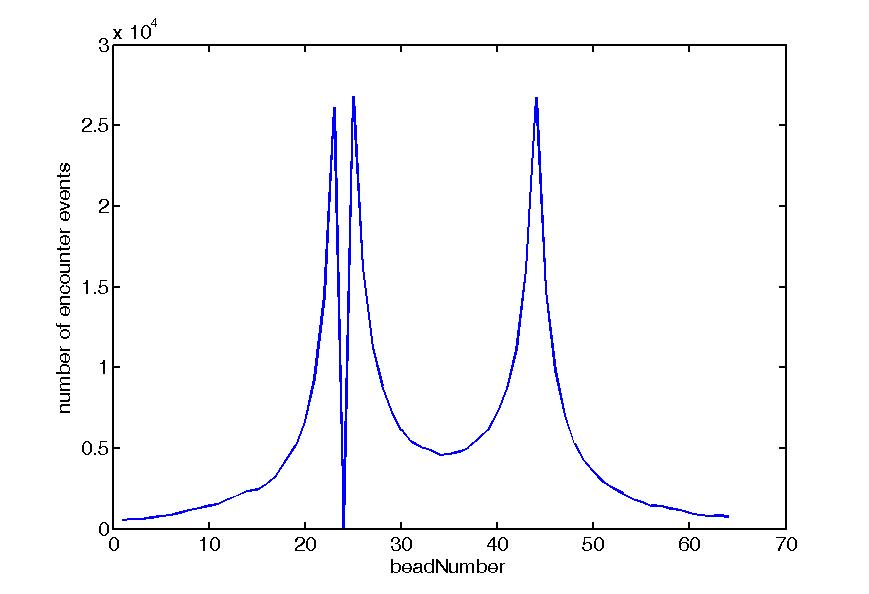
\includegraphics[scale=0.4]{encounterHistBead24connect24And44EncounterDist0_1}
\caption{\scriptsize{the encounter histogram of bead 24 as a function of bead number. The polymer included 64 beads with Kuhn length of 0.1, the encounter distance was set to be 0.1. the self encounters were trivially zeroed out}}
\label{figure_encounterHistBead24connect24And44EncounterDist0_1}
\end{figure}


\section{One, two and three loops at fixed positions}
Here we present \textit{in-silico} experimental results conducted for the case of fixed 1,2, and 3 loops, i.e. beads connected to form loops remain the same throughout the simulations. We use a polymer composed of 64 beads and sequentially simulate the model with loops between bead [10 19], [28 37] and [46 55] of the linear chain. For each case 10,000 simulations were performed.

The encounter histograms are presented in Figure \ref{figure_encounterHistogram123Loops} The mean encounter probability calculated for each case is shown in Figure \ref{figure_encounterHistogram123Loops}. The encounter data was fitted with a function of the form $\alpha x^{-\beta}$. The beta values are reported in the legend of Figure \ref{figure_encounterHistogram123Loops}. Since the loops length was set to 9, the encounter probability for the three cases, as a function of distance, shows an increase around distance 9. The values of the probability at that distance are 0.03, 0.034, and 0.035, for 1, 2 and 3 fixed loops respectively. 
\begin{figure}[H]
\centering
\hspace{-72pt}
\vspace{-40pt}
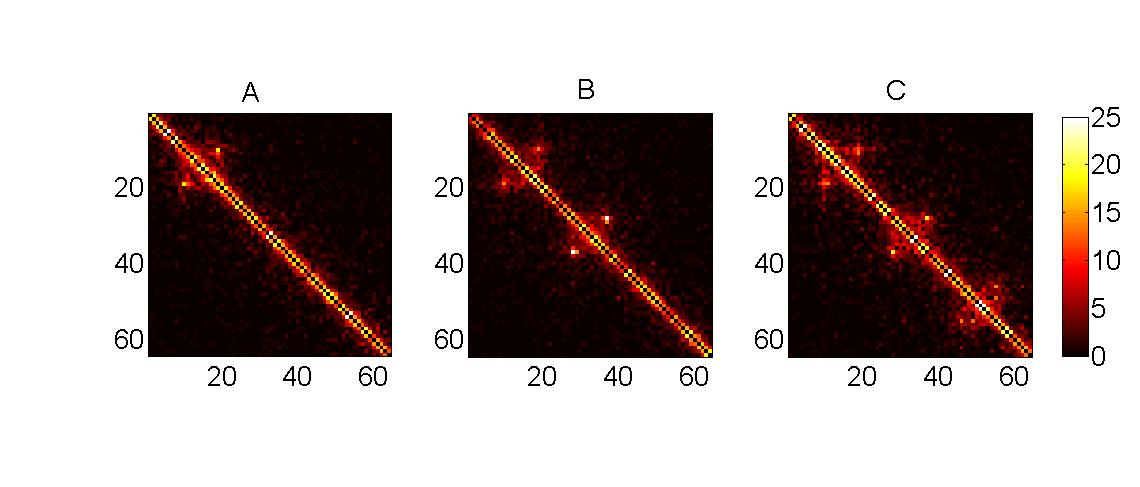
\includegraphics[scale=0.4]{encounterHistogram123Loops}
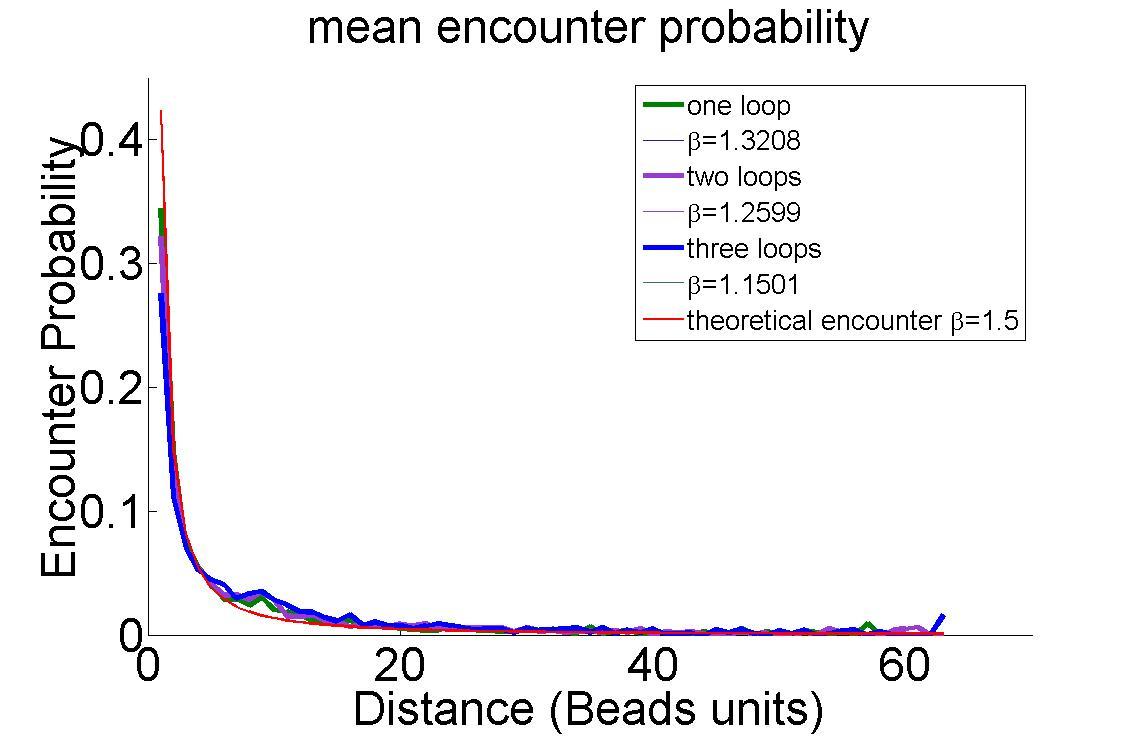
\includegraphics[scale=0.2]{meanEncounterProbability123Loops}
\caption{\scriptsize{The encounter histograms (upper panel) of the 3 fixed position loops cases. (A) a single loop between beads [10 19]. (B) two loops in [10 19], [28 37]. (C) three loops in [10 19],[28 37], and [46 55]]. Each point in the 64 by 64 matrices above represent number of encounters between bead $i$ and $j$. The mean encounter probability (lower panel) for the 3 fixed loops cases: one fixed loop (green), 2 fixed loops (purple), and 3 fixed loops (blue). The fitted $\beta$ values  for the 3 cases are reported in the legend. The theoretical encounter probability curve ($\beta=1.5$) is shown in red. The bump around distance 9 indicates shows the higher encounter probability for the three cases, since the length of each loop was set to 9.}}
\label{figure_encounterHistogram123Loops}
\end{figure}


\subsection{Internal loops}\label{subsection_internalLoops}
We now turn to examine the encounter probability of a model containing one 'big' loop when internal loops are sequentially added in it (see Figure \ref{figure_encounterHistogram1To10InternalLoops} lower right panel).  
That is, we connect bead $i$ and $j$ ($j>>i$) and add $n$ loops at of random lengths between bead $i+1$ and bead $j-1$, with the constraint that any bead cannot be connected to form more than one loop. 

For the results presented here, we chose the beads 5 and 60 to form the big loop, we perform 10 simulation rounds, in each we increase the number of internal loops from 1 to 10. The connected beads forming the internal loops are chosen at random. Encounter histogram for the 10 cases are shown in Figure \ref{figure_encounterHistogram1To10InternalLoops} (upper panel). As the number of internal loops is increased, the encounter probability between beads in the loop increases.

The calculated mean encounter probabilities  for the 10 cases are presented in Figure \ref{figure_encounterHistogram1To10InternalLoops} (lower left panel)
\begin{figure}[H]
\centering
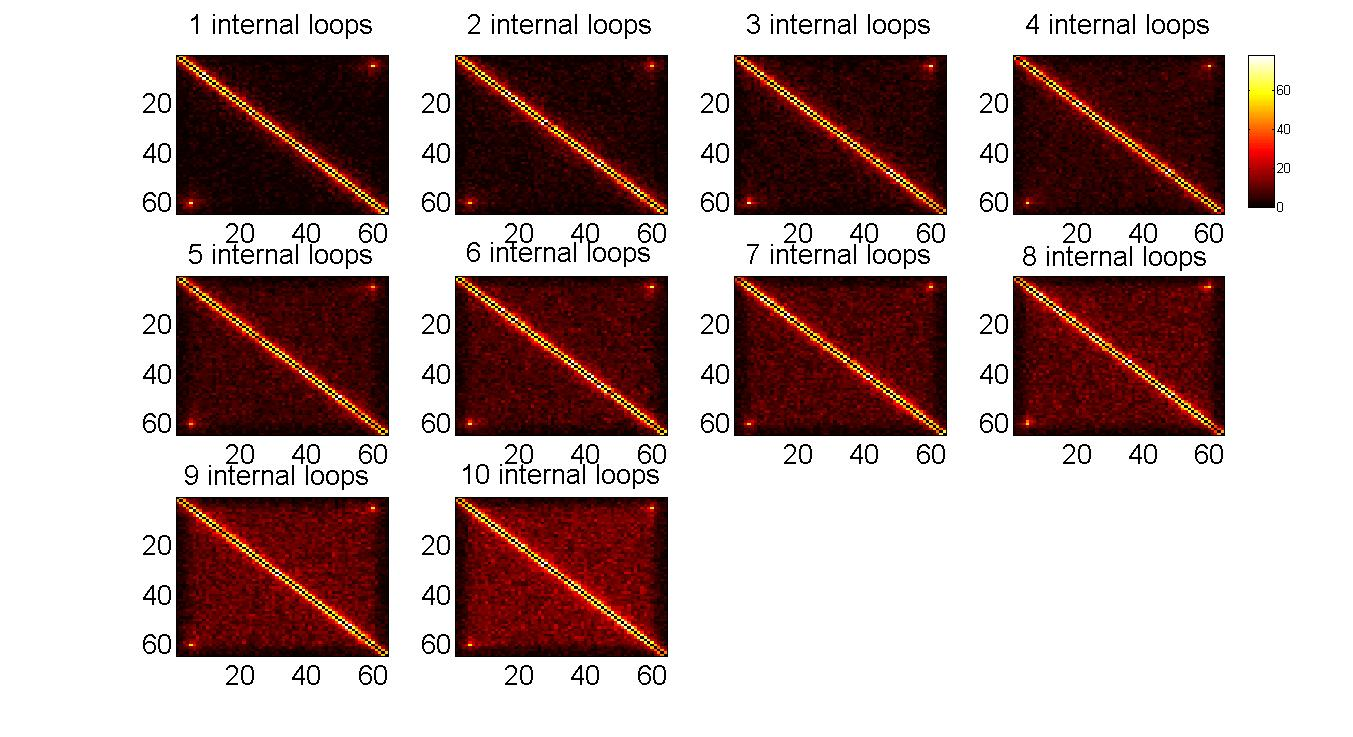
\includegraphics[scale=0.3]{encounterHistogram1To10InternalLoops}
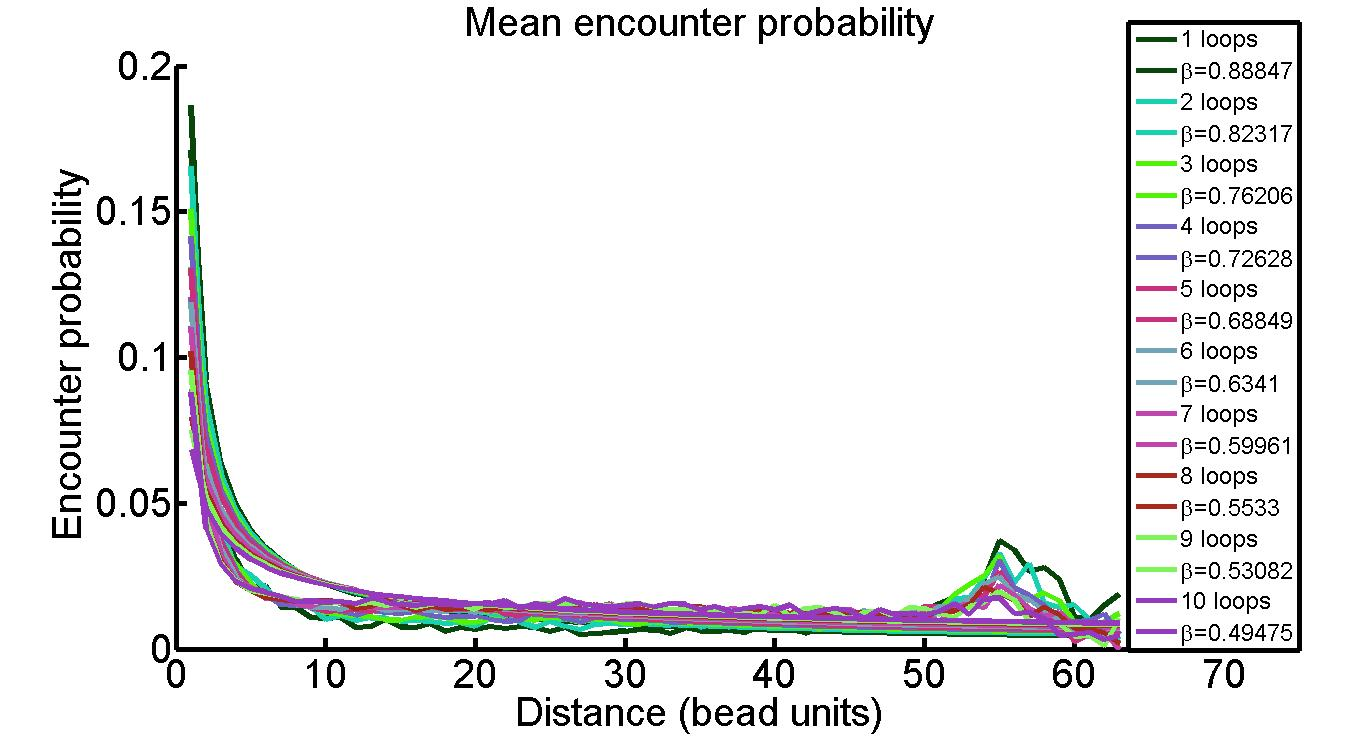
\includegraphics[scale=0.15]{meanEncounterProbabilityInternalLoops}
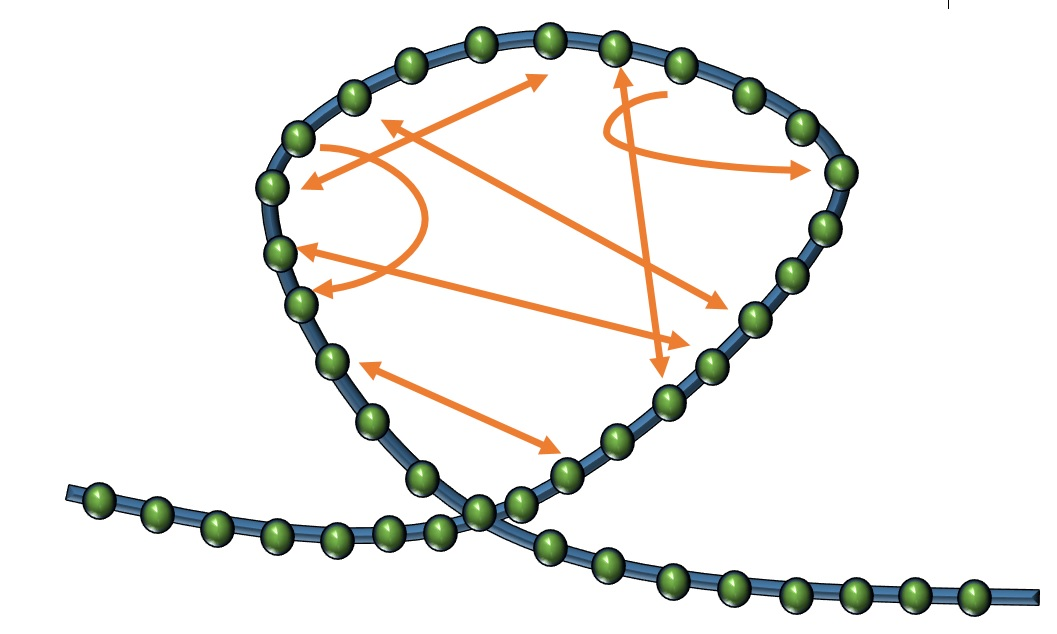
\includegraphics[scale=0.2]{polymerModelWithLoopAndInternalConnectors}
\caption{\scriptsize{The encounter histogram (upper panel) of the model with one big loop between beads 5 and 60, when 1 to 10 internal loops are added to it. The mean encounter probabilities curves (lower left panel) as the number of internal loops is increased from 1 to 10. The simulated encounter data was fitted with a function of the form $\alpha x^{-\beta}$,where $x=1..63$ is the distance in beads units. The bump in distance 55 represents the connection between bead 5 and 59, which constitute the 'big' loop in our simulations and is seen as a consistent bright spot in the encounter histogram (upper panel). A cartoon of the looped model (lower right panel) with internal loops ,arrows indicate the beads to be connected. In the simulation in \ref{subsection_internalLoops} we simulate the polymer in the loop region, without the tails}}
\label{figure_encounterHistogram1To10InternalLoops}
\end{figure}


\section{Random fixed loops}\label{section_RandomFixedLoops}
In this experiment we add random length loops between bead $i$ and $j$. We term the range of beads between $i$ and $j$ as a TAD. 

\subsection{One TAD}
To simulate a TAD, we employ the random fixed loop model and restrict the bead pairs forming the loops to take indices between beads 1 to 32, the second half of the chain remains a linear Rouse chain. No bead can participate in forming more than one loop. 
We sequentially add 1 to 8 random fixed loops in the region of the TAD, matching the case of 2 to 16 beads participating in loop formation. 

\begin{figure}[H]
\centering
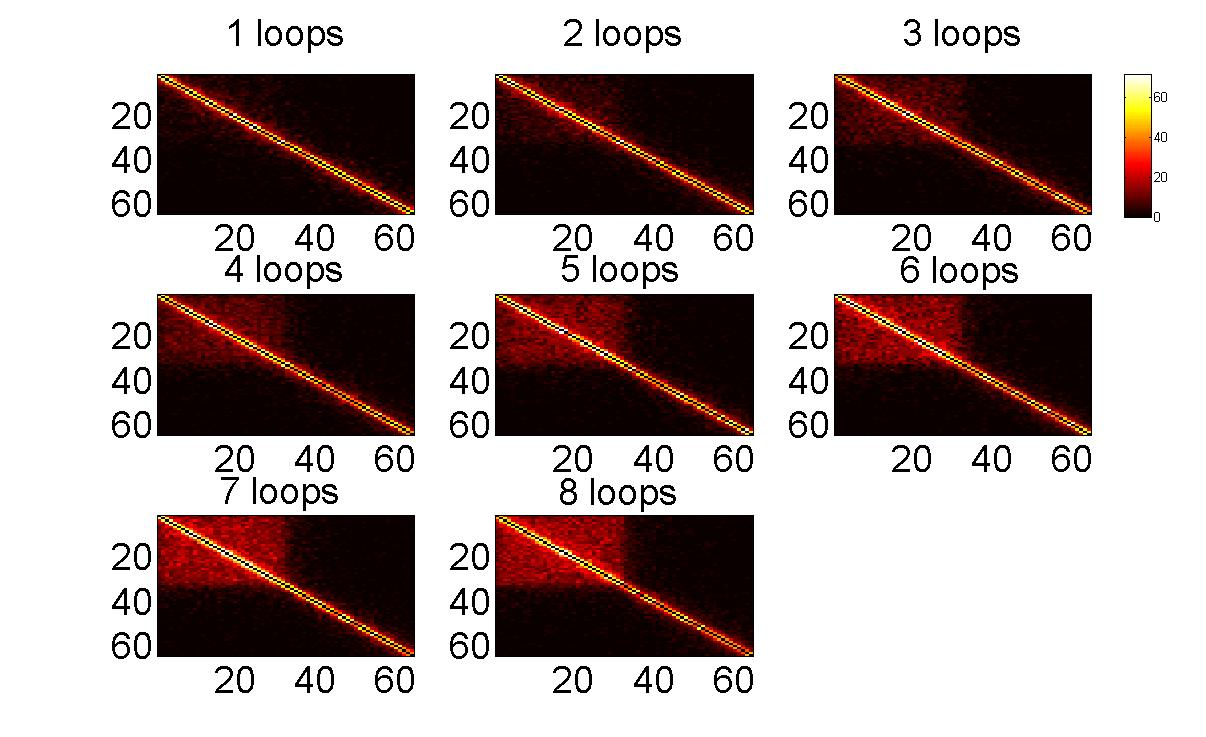
\includegraphics[scale=0.25]{encounterHistogram_1to8Loops}
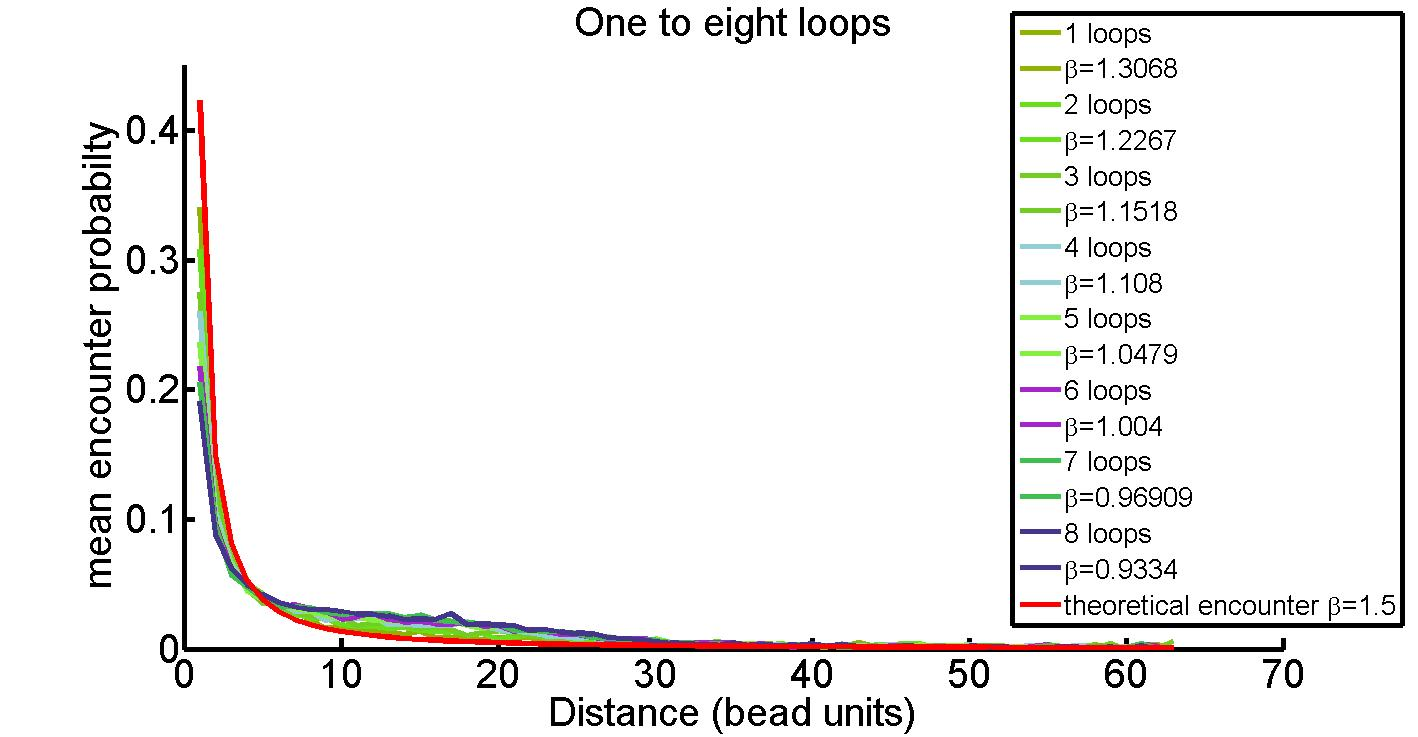
\includegraphics[scale=0.12]{meanEncounterProbabilityOneTAD1To8Loops}
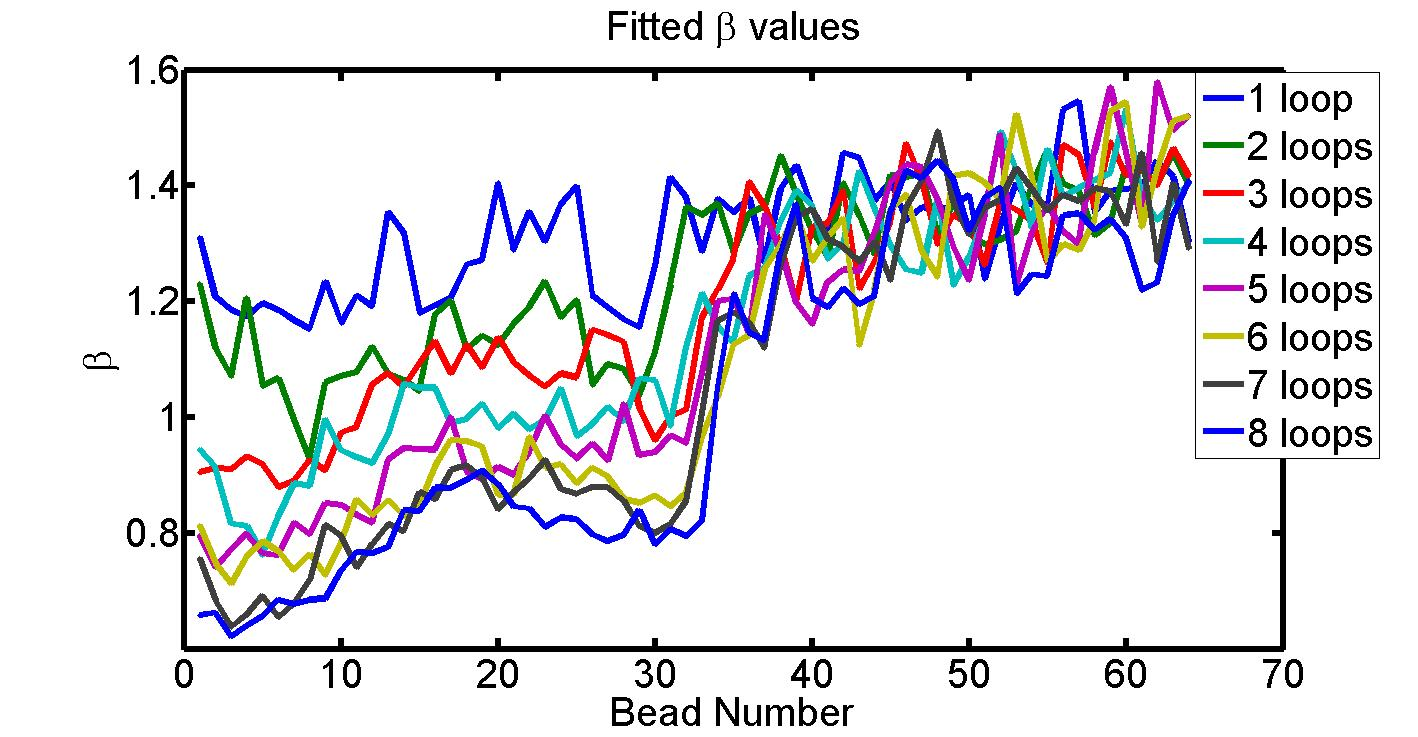
\includegraphics[scale=0.12]{fittedExpOneTAD1To8Loops}
\caption{\scriptsize{The encounter histogram (upper panel) of the case of random fixed loops in the region 1 to 32. As the number of random loops increases from 1 to 8 we see the emergance of a TAD region. The mean encounter probability (lower left panel) of the eight cases. The decrease in $\beta$ as the number of loops increases is attributed to the increased encounter between the first 32 beads. The fitted $\beta$ values (lower right panel) for the encounter data of each bead is displayed for the 8 cases.}}
\end{figure}

\subsection{Two TADS}
We follow similar procedure as with the one TAD simulation, only now we create random loops in two regions to form two TADs. The first regions is defined between bead 1 to 32, the second region between bead 33 to 64. In each simulation round we sequentially increase the number of random fixed loops from 1 to 10 (Figure \ref{figure_randomLoopModel1To10Loops64BeadsTwoTADs}). 

\begin{figure}[H]
\centering
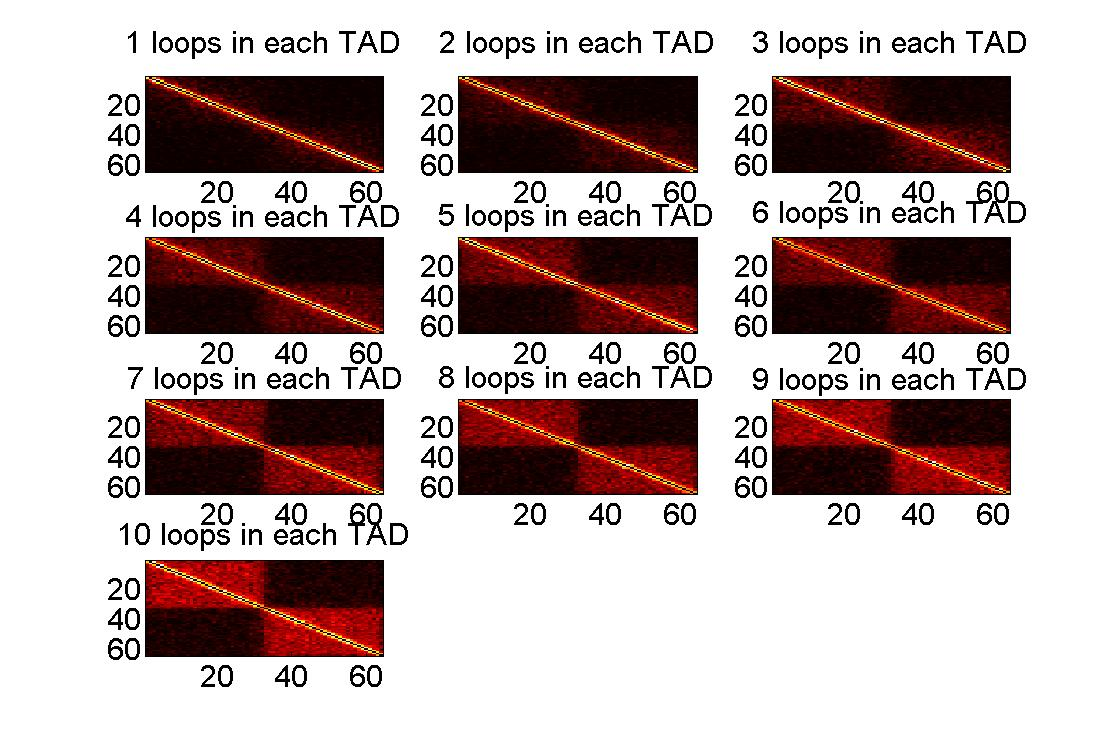
\includegraphics[scale=0.25]{encounterHistogram1To10LoopsInEachTAD}
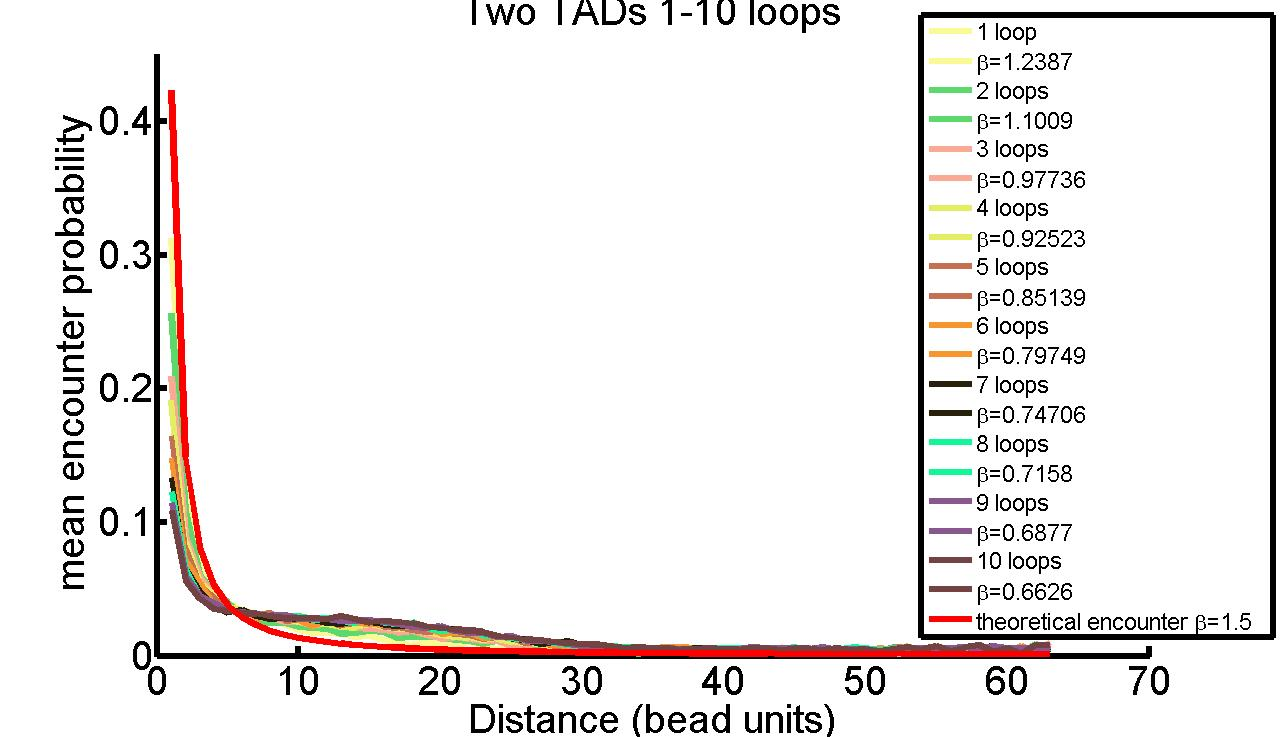
\includegraphics[scale=0.1]{meanEncounterProbabilityTwoTADs}
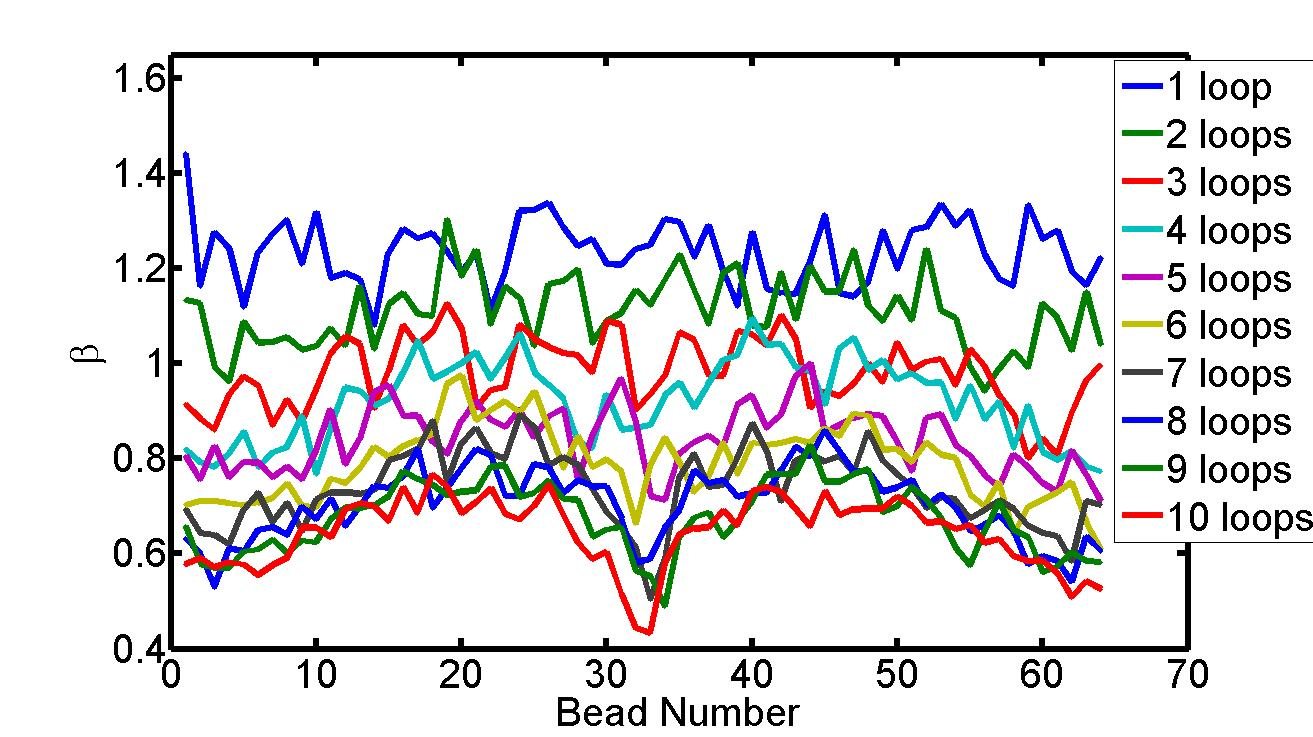
\includegraphics[scale=0.1]{fittedExpTwoTADs1To10Loops}
\caption{\scriptsize{The encounter histograms (upper panel) of the case with two TADs. As the number of loops in each TAD increases from 1 to 10, the two TADs emerges. The mean encounter probability (lower left panel) of the 10 cases resembles that of the one TAD case due to to 32 beads size of the TAD. The fitted $\beta$ values for the encounter probability of each bead in the 10 cases (lower right panel).}}
\label{figure_randomLoopModel1To10Loops64BeadsTwoTADs}
\end{figure}

\section{Simulation of variable loop number}
\subsection{One TAD}
To examine the effect of increasing the number of stable loops on the encounter probability, a chain of 32 beads was constructed. The number of stable loops varied from 0 to 16. the bond length $b=0.1$, the encounter distance was set to $b/2=0.05$, the time step was set to prevent simulation blow ups by the formula above, $\Delta t=8.3\times10^{-4}$. For each number of loops, random pairs of beads were chosen to be connected. 
\begin{figure}[H]
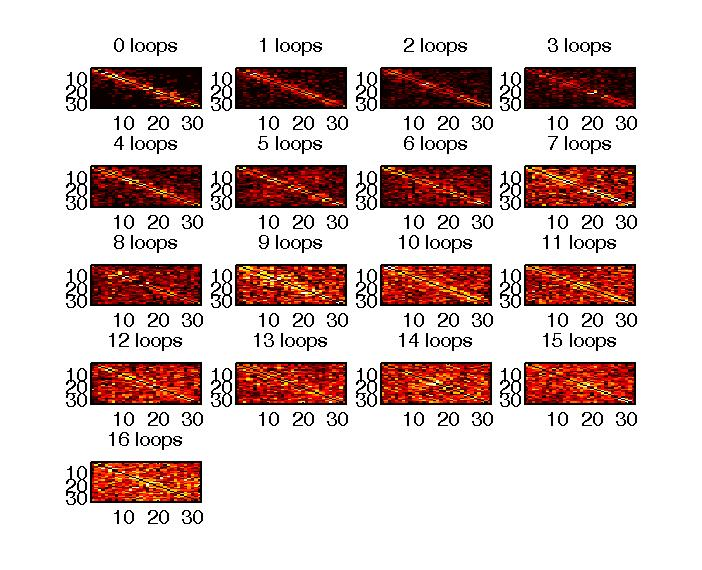
\includegraphics[scale=0.4]{stableLoopModelVariableLoopNumber32Beads}
\caption{\scriptsize{The encounter histogram of a chain of 32 beads. When the number of loops varies from 0 to 16 an area resembling a TAD emerges}}
\label{figure_stableLoopModelVariableLoopNumber32Beads}
\end{figure}

for each choice of loop number, we fit a curve to the encounter probability as a function of distance [beads].
\begin{figure}[H]
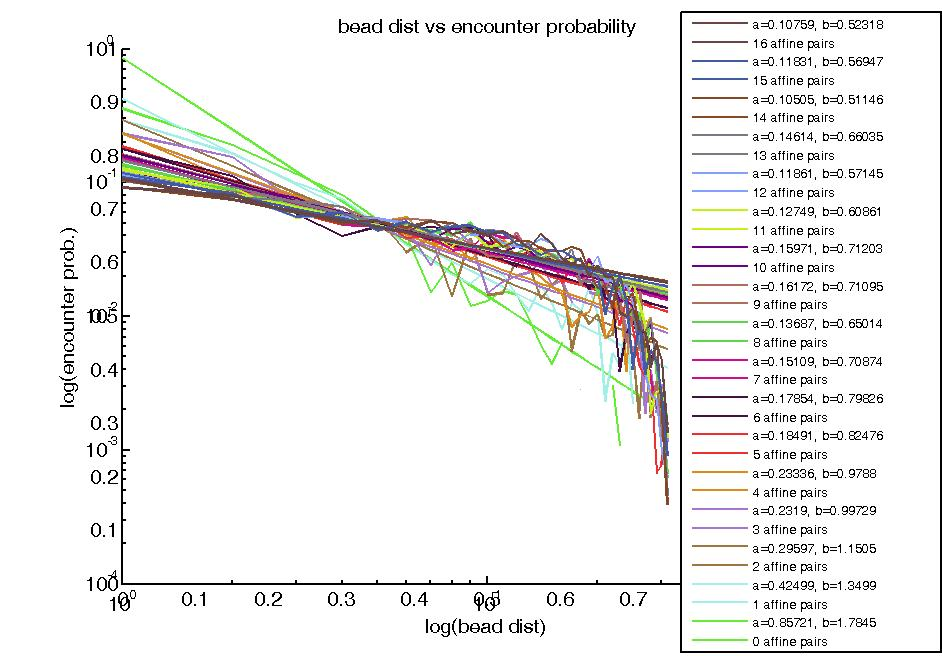
\includegraphics[scale=0.3]{logBeadDistanceVsEncounterProbabilityVariableLoops32Beads}
\label{figure_logBeadDistanceVsEncounterProbabilityVariableLoops32Bead}
\end{figure}

The fitted exponent values are decreasing roughly quadratically. 
\begin{figure}[H]
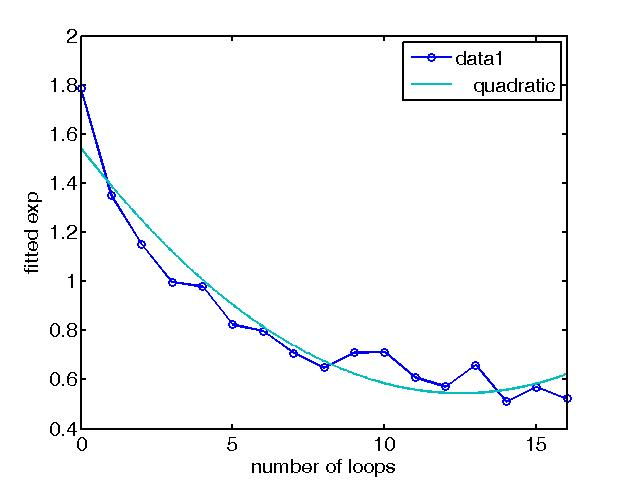
\includegraphics[scale=0.3]{changeOfExponentAsAfunctionOfLoopsStableLoopModelVariableLoops32Beads}
\label{figure_changeOfExponentAsAfunctionOfLoopsStableLoopModelVariableLoops32Beads}
\end{figure}
	
\subsubsection{One TAD with  a 'tail'}
In this simulation we test the affect of the increase in the number of stable loops on the bead encounter probability. An ensemble of chains comprised of 64 beads were simulated to $1.2$ times the relaxation time of the first Rouse mode, resulting in about $16,000$ steps for each chain. For each loop number 300 simulation were carried out. The bond length was set to be $b=0.1$, the encounter distance $\epsilon=b/2$, time step was set to be $\delta t=10^{-4}$. Stable loops were defined between bead $1$ and $32$ which we expect to resemble a TAD. At each simulation round we increase the number of loops $L$ by choosing at random $2L$ bead indexes of bead to be connected, $L$ is varied from 0 to 15. the encounter histogram shows an increasing encounter pattern in the region the loops are defined in (see Figure \ref{figure_stableLoopModelVariableLoopNumber64Beads})
 
\begin{figure}[H]
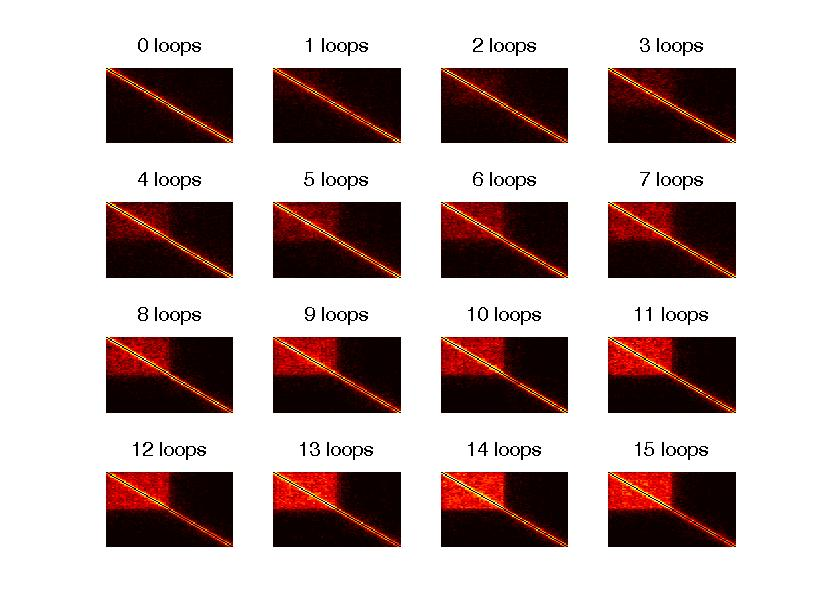
\includegraphics[scale=0.3]{stableLoopModelVariableLoopNumber64Beads}
\caption{\scriptsize{The affect of increasing the stable loops in a polymer of 64 beads. Loops were created at random between beads located in the first half of the polymer. Increasing the number of loops from 0 to 15 reveals a region resembling a TAD as seen in the data}}
\label{figure_stableLoopModelVariableLoopNumber64Beads}
\end{figure} 
 
 The encounter probabilities for the chains when increasing the loops from 0 to 15, can be seen in Figure \ref{figure_logBeadDistanceVsEncounterProbabilityVariableLoops64Beads}
For each encounter probability curve we fit a function of the form $ad^{-b}$. The change in the exponent $b$ as a function of the number of loops is seen in Figure \ref{figure_changeOfExponentAsAfunctionOfLoopsStableLoopModelVariableLoops64Beads}

\begin{figure}[H]
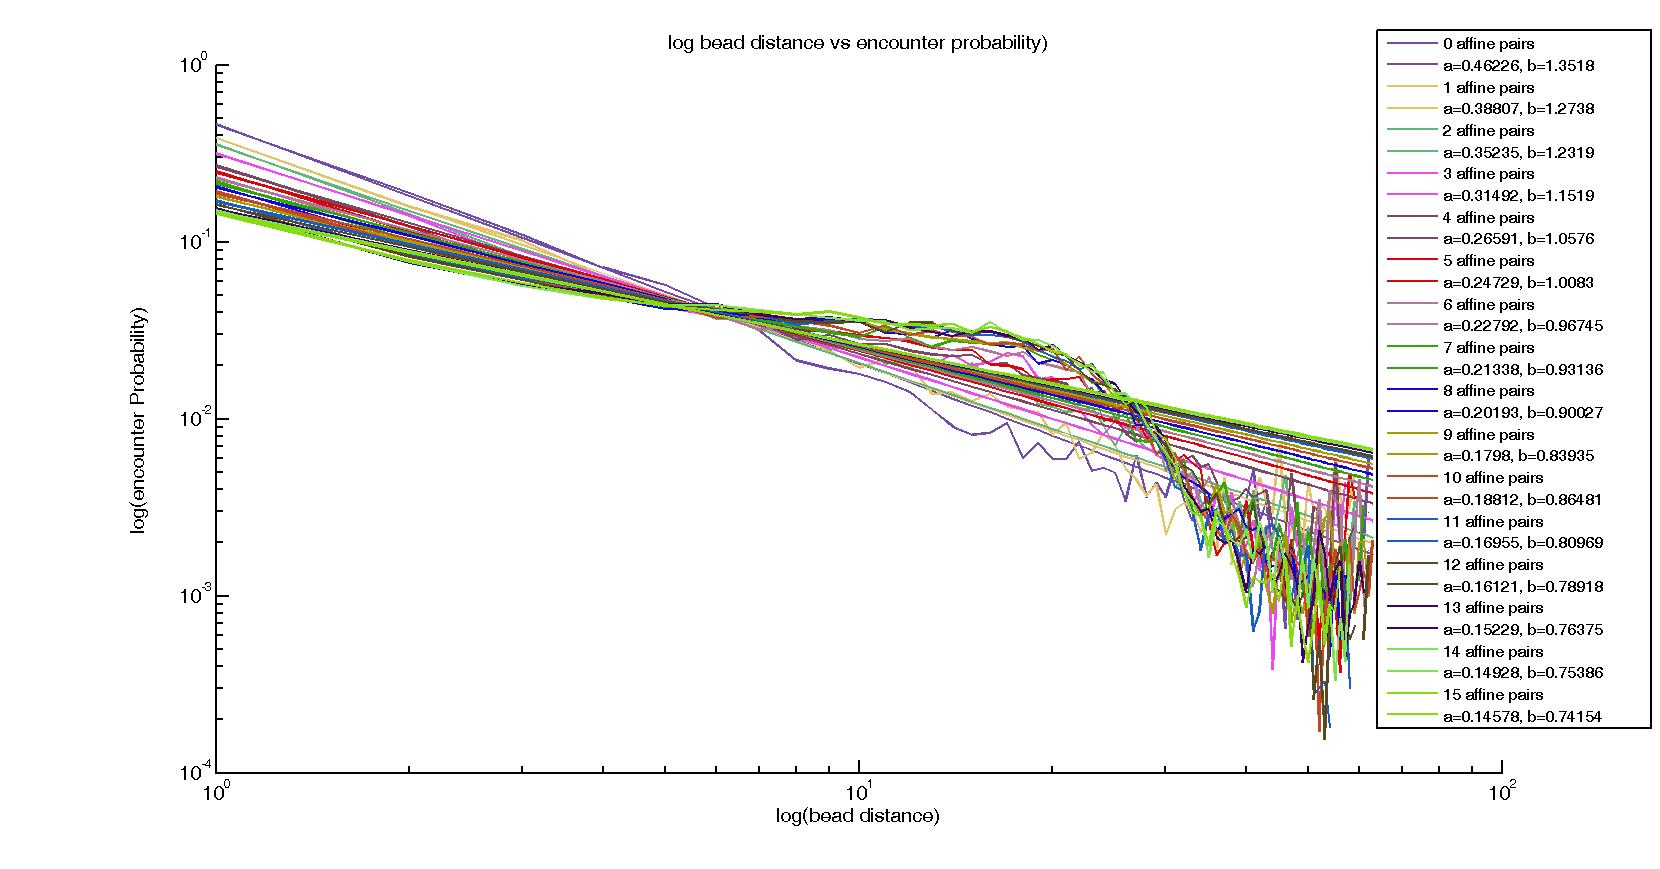
\includegraphics[scale=0.2]{logBeadDistanceVsEncounterProbabilityVariableLoops64Beads}
\caption{\scriptsize{Encounter probability vs bead distance for the 16 models representing variable stable loops number if the first half of the chain of 64 beads (top)}}
\label{figure_logBeadDistanceVsEncounterProbabilityVariableLoops64Beads}
\end{figure}

\begin{figure}[H]
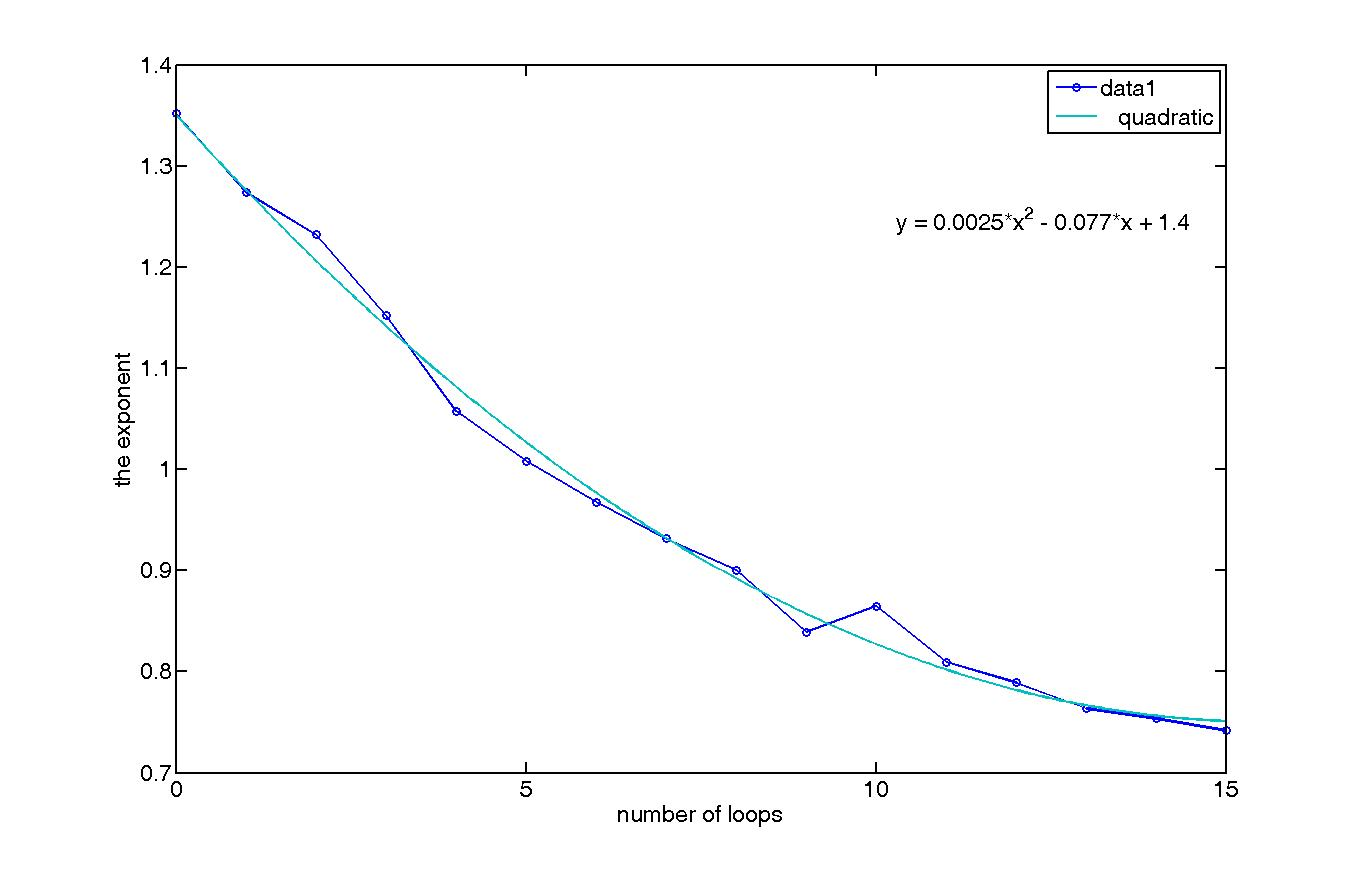
\includegraphics[scale=0.15]{changeOfExponentAsAfunctionOfLoopsStableLoopModelVariableLoops64Beads}
\caption{\scriptsize{The change in the value of the fitted exponent to the encounter probability curves of models with increasing number of stable loops. The decrease in the values of $b$ quadratic as can be seen by the cyan line fitted to the data.}}
\label{figure_changeOfExponentAsAfunctionOfLoopsStableLoopModelVariableLoops64Beads}
\end{figure}
\subsection{Two TADs}
 % unfinished

\section{Dynamic loop model}\label{section_dynamicLoopModel}
It can be assumed that stiff fixed loops in the chromatin are not always stable, but can open and close transiently. We turn to examine whether a model with loops that can be formed, held fixed, for some period, and be released, can explain the appearance of the TADS. The rational behind is that the variability of cells used in the experiments some in different states, i,e. are found with different initial chromatin loops. When these cells are fixed and the chromatin is cross-linked, the cross-links that will be formed will depend on the proximity of the beads conditional on the loops present at the moment the experiment began. 


A polymer with 128 beads was simulated. We define two region with high affinity of their member beads to a specific point in them. These regions can be considered as the TADs. Each region is of size $25$ beads. The first region is defined to be from bead 1 to 25, the second from bead $77$ to $102$. 

To simulate the state of experiment initiation, we define two beads in each TAD, which have high probability to be found together, and run simulations until steady state. Only one pair from each TAD was examined in each simulation, which we vary from simulation to simulation. At the end of each simulation we retrieve the encounters frequency for all the beads. 

Beads that come in close proximity to one another, are considered attached, and can be released and some rate $k_{off}$. The attachment distance was defined as half of the connector length between adjacent beads. 

\begin{figure}[H]
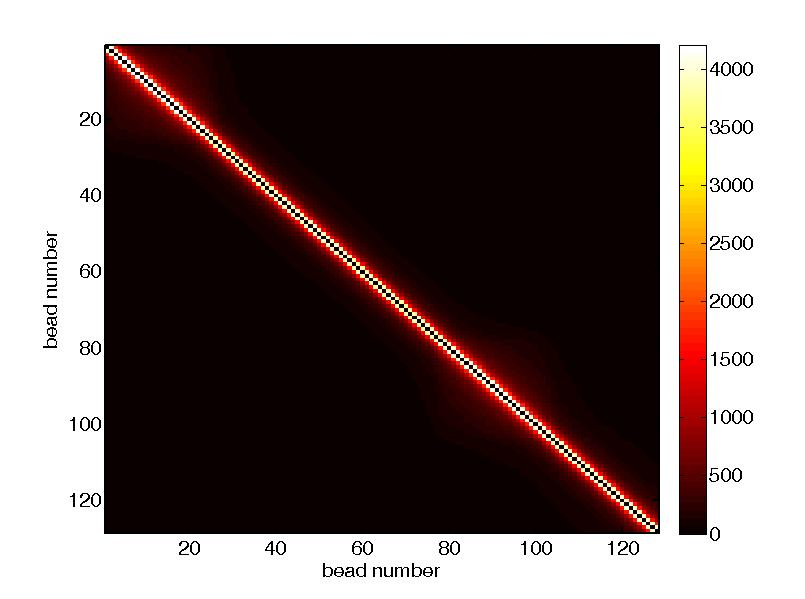
\includegraphics[scale=0.2]{encounterFrequency128beadsWithTadTransientModel}
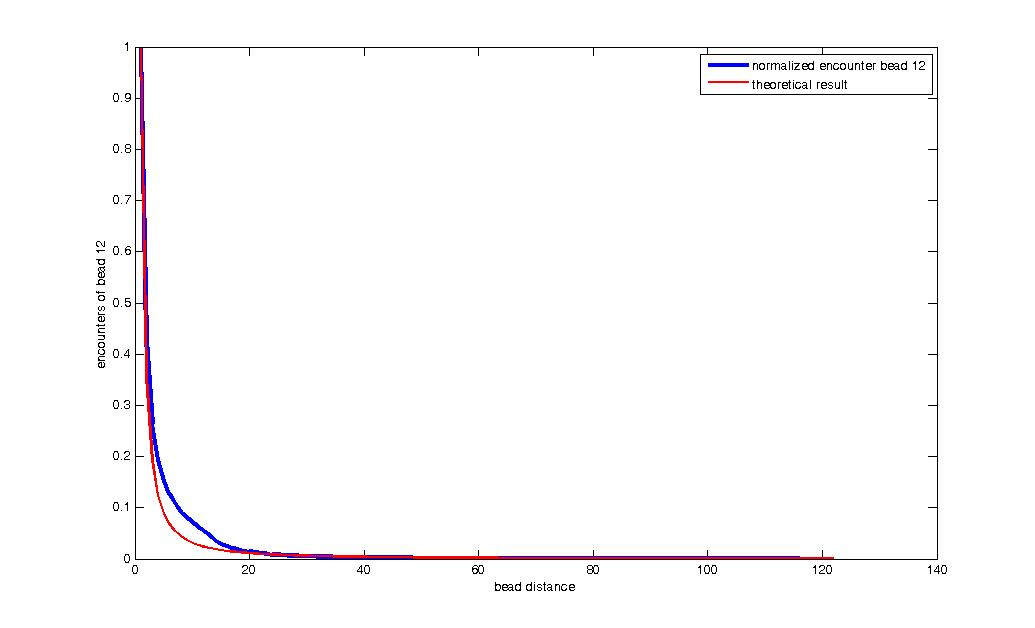
\includegraphics[scale=0.2]{encounterCrossectionBead12TransientLoopModelwithTheoreticalCurve}
\caption{\scriptsize{The mean encounter matrix for the transient loop model. the chain included 128 beads, with connector length of 0.1. Two regions were defined as the TADs: Bead 1 to bead 25, and bead 77 to 102. at each simulation, a pair of beads from each region were considered as having some affinity to one another. The model was simulated for each choice of affine pair until steady-state, 30000 steps. The mean encounter of all simulation in presented.}} 
\end{figure}

For beads that are not affine to any other, like the beads 26 to 77, the encounter frequency retrieved matches the theoretical result. 

\section{TAD D and E with cross-links corresponding to the peaks of the experimental data}
We next wanted to verify whether using a Rouse polymer and connecting beads for which the peaks of the experimental data, would allow us to reproduce the TADs. 

A polymer with 307 beads was created, corresponding to the TAD D (107 beads) and E (200 beads). The cross-links were made at the mid point of bead numbers displayed in Table \ref{nonNeighborBeadEncounterTable}. Thirty simulations were performed and their average distance matrix after relaxation time is presented in Figure \ref{figure_meanEncounterMatrixOfSimulatingTADEandDWithLoops}. As can be seen the location of the cross-links create 'hot spots' in the mean distance matrix. In comparison to Figure \ref{TADsOfTheXChromosome}, we see that there is little resemblance. Thus concluding that creating cross-links according to the encounter matrix, is not sufficient to reproduce the TADs.

\begin{figure}[H]
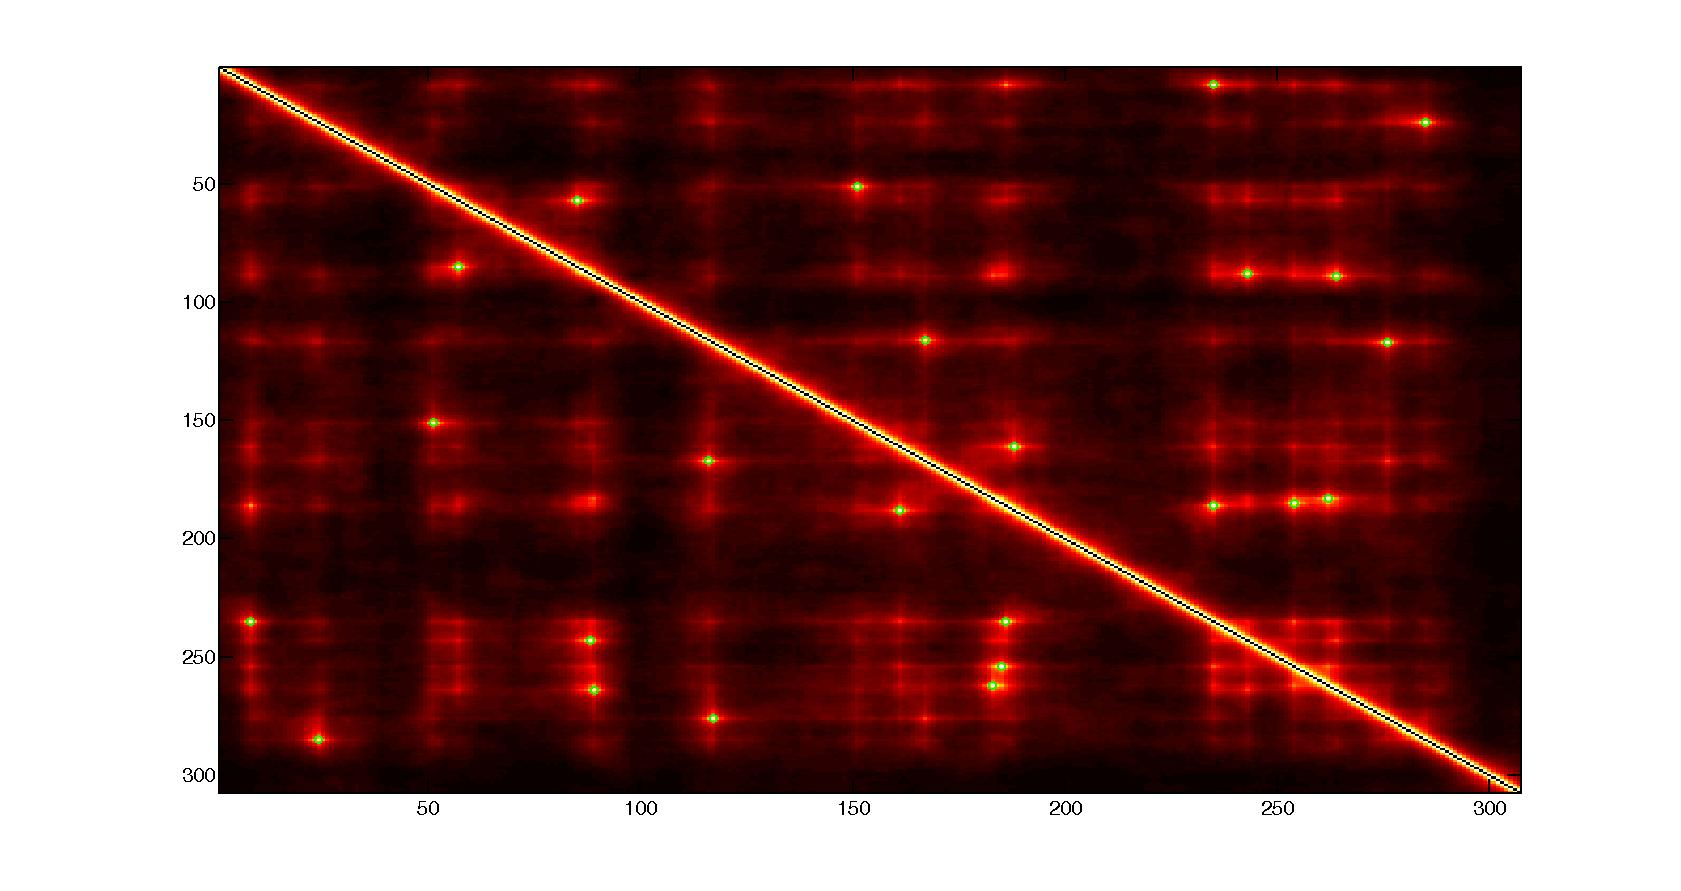
\includegraphics[scale=0.2]{meanEncounterMatrixOfSimulatingTADEandDWithLoops}
\caption{\scriptsize{The mean of 30 simulation of the polymer with 307 beads, connected corresponding to the peaks of the encounter data (Luca et al). The small green circles represent locations of connected bead pairs. These circles overlap with peaks of the simulated encounter matrix. It is evident that the TAD structure was not reproduced with this approach. The x and y axes  represent bead numbers. Each pixel represents the encounter number of bead $i$ and $j$}}
\label{figure_meanEncounterMatrixOfSimulatingTADEandDWithLoops}
\end{figure}

\section{Conditional encounter probability}

\subsection{Three beads in a linear chain}\label{subsection_conditionalEncounter3BeadsInALinearChain}

In the analysis of the experimental data as performed by Giorgetti et al\cite{giorgetti2014predictive}, 3 loci were found to be significant to the internal organization of TAD D. These loci overlap the position of the highly interacting Xite/Tsix, Chic1, and Linx, which correspond to beads in the range 25-27, 33-35, and 86-89 respectively.

We therefore simulate a 108 beads chain and assess the conditional probability that  bead 34 (Chic1) encounter bead 26 (Xite/Tsix) before bead 87 (Linx). All simulations were ran until an encounter occurred. Time step was set to $8.3\times 10^{-5}$ [sec]. The encounter distance was set to $b/5=0.02$, where $b$ is the standard-deviation of the distance between adjacent beads. 

The conditional encounter probability is summarized in the following table 
\begin{table}[H]
\begin{tabular}{l |c| c |c |}
 prob loci                    & bead num.           & prob & MFET [sec]\\
\hline
 Chic1$\rightarrow$ Xite/Tsix & 34$\rightarrow$ 26  & 0.9378 & 0.2273\\
 Chic1 $\rightarrow$ Linx     & 34 $\rightarrow$ 87 & 0.0622 & 0.1903
\end{tabular}
\end{table}
Not that we work in units of $k_BT$, hence the times should be multiplied by this factor. 

\subsection{Two beads in the random fixed loops model}\label{subsection_conditionalEncounter2BeadsInTheRandomFixedLoopModel}
Next, we examine the conditional encounter probability of the 3 loci (beads 26,34, and 87) in the context of the random fixed loops model as described in subsection \ref{section_RandomFixedLoops}. To simulate the D TAD, we use a chain of 108 beads, and run 10,000 simulations with a time step of $8.3\times 10^{-5}$ [sec], and an encounter distance of $b/5=0.02$. We set 10 randomly placed fixed loops for each simulation, where the beads 26, 34, and 87 are prohibited from forming loops. The conditional probability of bead 34 meeting bead 26 before it meats bead 87 is summarized Table \ref{table_conditionalEncounterDynamicLoop} along with the mean first encounter time.

\begin{table}[H]

\begin{tabular}{l | c| c| c|}
 prob loci & bead num. &prob & MFET [sec]\\
\hline
 Chic1$\rightarrow$ Xite/Tsix & 34 $\rightarrow$ 26   & 0.725 & 0.1154\\
 Chic1 $\rightarrow$ Linx     & 34 $\rightarrow$ 87  & 0.275 & 0.1422	
 \end{tabular}
 \caption{}\label{table_conditionalEncounterDynamicLoop}
\end{table}

\subsection{Two beads and a loop}\label{subsection_conditionalEncounter2BeadsAndALoop}
We now turn to explore the conditional probability that a bead $B$ encounters bead $A$ before it encounter bead $C$ in a chain containing one loop. There are 27 configurations for the position of the beads in relation to the loop. Here we address the case of a chain with two equally sized tails. Thus, due to symmetry we reduce the possible configurations to 14. We term the beads contained in the loop as \textit{in the loop} and beads outside as beads \textit{on the tail}. The possible configurations are: 
\begin{enumerate}
 \itemsep1pt \parsep0pt \parskip1pt 
\item $A$ in the loop, $B$ and $C$ on the same tail
\item $A$ in the loop, $B$ and $C$ on different tails
\item $B$ in the loop, $A$ and $C$ on the same tail
\item $B$ in the loop, $A$ and $C$ on different tails
\item $C$ in the loop, $A$ and $B$ on the same tail 
\item $C$ in the loop, $A$ and $B$ on different tails 
\item $A$ and $B$ in the loop, $C$ on the tail 
\item $A$ and $C$ in the loop, $B$ on the tail 
\item $B$ and $C$ in the loop, $A$ on the tail 
\item $A$, $B$ and $C$ in the loop
\item $A$, $B$ and $C$ are on the tail
\item $A$, $B$ on one tail, $C$ on the other tail
\item $A$, $C$ on one tail, $B$ on the other tail
\item $B$, $C$ on one tail, $A$ on the other tail
\end{enumerate}
The different cases are summarized graphically in Figure \ref{figure_possibleArrangementOfThreeBeadsAndAloop}
\begin{figure}[H]
 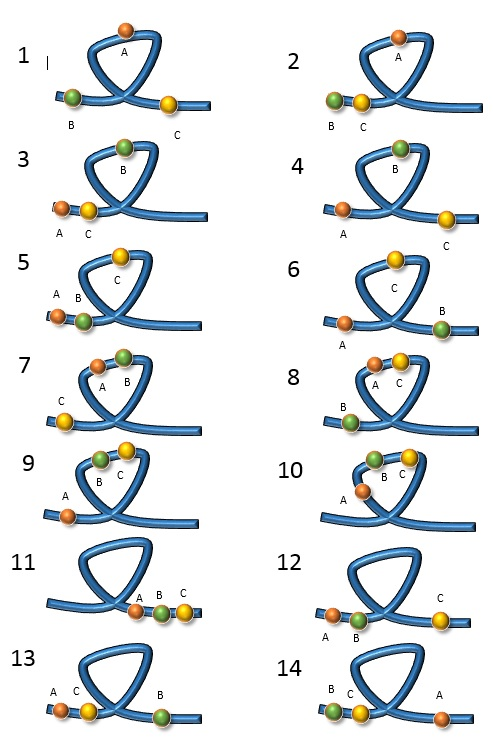
\includegraphics[scale=0.5]{possibleArrangementOfThreeBeadsAndAloop.jpg}
 \caption{\scriptsize{The possible configuration in the case of three beads and a loop, leaving tails of equal length}}\label{figure_possibleArrangementOfThreeBeadsAndAloop}
\end{figure}

The conditional probability encounters and the mean first encounter time, are summarized in the Table \ref{table_conditionalEncouterProbabilityAndMFET}
according to the cases specified above
\begin{table}[H]

\begin{tabular}{l|l|l|l|l}
case & Bead A-B & MFET A-B (sec)&Bead B-C & MFET B-C (sec)\\
 \hline
1 & 0.15 & 0.34 & 0.85 & 0.23\\
2 & 0.76 & 3.97 & 0.23 & 3.11\\
3 & 0.37 & 1.47 & 0.63 & 1.46\\
4 & 0.53 & 1.79 & 0.47 & 2.25\\
5 & 0.86 & 0.29 & 0.16 & 0.15\\
6 & 0.29 & 2.57 & 0.71 & 4.14\\
7 & 0.79 & 0.55 & 0.21 & 0.45\\
8 & 0.63 & 1.83 & 0.37 & 2.20\\
9 & 0.26 & 0.46 & 0.74 & 0.81\\
10& 0.52 & 0.13 & 0.48 & 0.15\\
11& 0.54 & 0.14 & 0.46 & 0.11\\
12& 0.97 & 0.29 & 0.03 & 0.13\\
13& 0.56 & 8.39 & 0.44 & 6.19\\
14& 0.01 & 0.02 & 0.99 & 0.3
\end{tabular}
\caption{\scriptsize{Summary of the results of simulating the conditional probability that bead B meets A before C (Bead A-B), and probability that bead B meets C before A (Bead B-C), with the mean first encounter time (MFET) given in units of seconds. For each cse 10 simulation were performed}}\label{table_conditionalEncouterProbabilityAndMFET}
\end{table} 

\chapter{Review of Literature}\label{chapter_reviewOfLiterature}
Here we give several key points from articles bearing important principals from the understanding of chromosome internal interaction and organization 

\section{From Nora et.al 2012 \cite{nora2012spatial}}
\begin{itemize}
 \itemsep1pt \parsep0pt \parskip1pt 
\item The X inactivation center (Xic) orchestrate the initiation of the X chromosome inactivation by controlling the expression of non-protein-coding Xist transcript. 
\item 5C techniques were  used to analyze the \textit{spatial} organization of the region including the Xist. The region analyzed  is 4.5 Mb in size. 
\item 200 kb to 1 Mb regions were discovered and named TAD.
\item TADs remain consistent between male and female Embryonic stem cells (ESC) and betwee different cell lines.
\item TADs remain persistent before and after cell differentiation and before and after X inactivation. Internal TAD connections remain high even after X inactivation. However, the intra-TAD connection are lower than those of the same TAD on the active X.
\item on the inactive X, the long range interaction($>50kb$) inside the TAD are lost. 
\item disrupting the regions between TADs caused an ectopic chromosomal contacts 
\item 5C-Forward and 5C-Reverse oligonucleotides were designed to conduct test on undifferentiated mouse embryonic stem cells (ESCs)
\item it was found that long range contacts (>50kb) happen within a series of discrete genomic blocks , roughly 0.2-1 Mb in size 
\item The chromosomal domains are self-associating. 
\item FISH experiment on 3D chromosomal conformation were conducted to verify the results.
\item in the FISH, the distance between probes lying in the same 5C domain were significantly shorter than of probes lying in different domains. 
\item a strong correlation was found between 5C count and 3D distance. 
\item bacterial artificial chromosome probes showed in experiments that large DNA segments belonging to the same 5C domain co-localize much more than DNA segment on adjacent domains \textit{throughout cell cycle}. 
\item a correlation was shown between the existence of H3K27me and the TADs. However, for a mouse with a knockout of these proteins, a significant change was \textit{not} observed in the composition and size of the TADs.
\item it was shown that H3K27me - an antibody signifying the presence of Histone 3- is not related to the folding of the genomic regions into TADs. 
\item when the boundary between TAD E and D (which include the Xist and Tsix), ectopic folding of TAD E was observed. It was assumed that boundary elements have an influence on the conformation of the TADs. 
\item after removing boundary elements between TADs, the TADs did not merge completely, hence concluded that there are other, intra-TADs element that control conformation.
\item TAD did not change during cell differentiation (from embryonic stem cell to neuronal progenitor and embryonic fibroblast), but the \textit{internal} connections inside each TAD did change.
\item for the TADs that did change, some have become \href{http://www.nature.com/nature/journal/v453/n7197/full/nature06947.html}{Lamina Associated Domains} (LADs) 
\item the transcription dynamics showed positive correlation for TADs for which the promoter of the genes was located inside the TAD. 
\item the correlation between gene expression of genes in the same TAD did not depend on the distance between genes in the TAD. 
\end{itemize}

\section{From Dekker et al 2013 \cite{dekker2013exploring}}
\begin{enumerate}
 \itemsep1pt \parsep0pt \parskip1pt 
\item This is a review of methods to analyze Chromosome Capture data and to infer mechanical properties of the DNA.
\item The 3C methods determines the encounter frequency of genomic segments, probably in the range of $10-100nm$
\item Chromosome are highly variable among cells \cite{muller2010stable}
\item There are some organizational principals at the scale of the whole nucleus
\item chromosomes occupy separate territories that do not usually mix\cite{marshall1997interphase}. When they do mix, they can potentially create functional interactions between loci on different chromosomes. 
\item transcription does not occur diffusively throughout the nucleus, but happen at sub-nuclear sites enriched in components of the transcription and RNA processing machinery.
\item Therefore, actively transcribed genes tend to co-localize
\item transcriptionally inactive segments tend to associate with each other and can often be found localized at the nuclear periphery
\item sub-nuclear positioning of the loci is correlated with gene expression
\item imaging approaches do not allow analysis of the 3D folding of a complete genome at the kb resolution. 
\item the 3C based methods do not distinguish functional from non-functional association of loci
\item the loci encounter frequency is affected by \begin{enumerate}
\item direct loci encounter
\item encounters mediated by proteins
\item indirect co-localization to the same sub-nuclear structure (e.g lamina)
\item result of chromosome packing and folding 
\item random encounters
\item interactions defined by the polymer physical characteristics
\end{enumerate}
\item the 3D chromatin is highly variable even among identical cells\cite{marshall1997interphase}.
\item analytical tools to interpret the 3c data focus first on specific point by-point looping interactions, e.g. between promoters and gene regulatory elements
\item in previous article, thousands of long range ($>4mb$) interactions were identified between promoters and enhancer-like regions \cite{sanyal2012long}
\item one abundant class of long range interaction involves promoters looping to sites bound by the \href{http://en.wikipedia.org/wiki/Insulator_(genetics)}{insulator protein} \href{http://en.wikipedia.org/wiki/CTCF}{CTCF}. The hypothesis is that these looping events have architectural role. 
\item genes are regulated by multiple distal elements \cite{gerstein2012architecture}
\item average pattern of looping interactions around promoters is asymmetric. Looping interaction are most frequently observed $\sim120kn$ upstream
\item human and mouse genome are each composed of over 2000 TADs covering $90\%$ of the genome.
\item TADs are defined by genetically encoded boundary elements \cite{nora2012spatial}.
\item boundary elements are enriched with CTCF-bound loci
\item the mechanisms that establish TAD boundaries are still unclear. 
\item analysis of mouse genome suggests tat enhancer-promoter interactions are particularly frequent within TADs \cite{shen2012map}
\item genes within the same TAD tend to be coordinately expressed during cell differentiation \cite{nora2012spatial}. Possibly because those genes share the same set of regulatory elements. 
\item the 3D structure of the Igh locus was inferred by polymer modeling and genome tagging to give discrete areas of looping \cite{jhunjhunwala20083d}.
\item the 3D structure of bacterial genome was determined by a combination of 5C data, imaging and modeling \cite{umbarger2011three}
\item in yeast it was demonstrated that a small set of spatial constraints is sufficient to yield a highly organized genome structure, i.e volume exclusion \cite{tjong2012physical}
\item HiC data shows lack of specific interactions for loci $>1Mb$ apart
\item HiC data for non-synchronized human cells show 3 regimes, each exhibiting a power law decline in the contact probability $P(s)\sim s^{-\alpha}$. for $s<0.7Mb$ $\alpha\approx0.7$, corresponding to the TADs. For $0.7Mb<s<10Mb$, $\alpha\approx1$. For $s>10Mb$, $\alpha$ is not well measures due to poor statistics \cite{lieberman2009comprehensive}.
\item a polymer model with excluded volume can give rise to an encounter probability with $\alpha=1$
\item 
\end{enumerate}

\section{The Hierarchy of the 3D genome.  Gibcus 2013 \cite{gibcus2013hierarchy}}
\begin{enumerate}
 \itemsep1pt \parsep0pt \parskip1pt 
\item neighboring chromosomes can overlap considerably 
\item the nuclear envelope (double lipid bilayer) restricts genomic DNA to confined 3D space and provides a solid anchor point that allows for specific chromatin interactions. 
\item The nuclear lamina is the inner nucleus membrane is associated with inactive heterochromatic chromatin directly or indirectly via lamina associated proteins.
\item almost half of the genome in a given cell population is composed of lamina associated domains \cite{guelen2008domain}. 
\item activated genes move to the nuclear interior and inactive genes are found in the lamina associated domains
\item loci gather near sub-nuclear structures such as the nucleoli, which are sub-nuclear structures dedicated to expression by RNA polymerase I. 
\item it has been shown that open, gene rich, areas and closed, gene-poor chromosomal domain are generally located in separate sub-nuclear regions \cite{fraser2007nuclear}
\item sub-chromosomal compartment were detected, named A and B, according to functional compartmentalization of gene activity \cite{lieberman2009comprehensive}. 
\item this compartmentalization is related to the association of loci to transcription factories and the nuclear lamina.  
\item loci found clustered in the A compartment are generally gene rich, transcriptionally active and DNase I hypersensitive 
\item loci found clustered in the B compartment are generally gen poor, transcriptionally silent, and DNase I insensitive \cite{lieberman2009comprehensive}.
\item those compartments are cell type specific, and cannot be predicted according to gene density. 
\item Chromatin domains preferentially associate with other domains of a comparable activity level.
\item The actively transcribed genes colocalize at foci called \href{http://en.wikipedia.org/wiki/Transcription_factories}{transcription factories}
\item groups of active genes, sometimes from different chromosome are found in these foci, enriched in the activity of RNA polymerase and other transcription factors.
\item genes located within the same TAD tend to have coordinated dynamics of expression during differentiation
\item so far TADs have not been described in bacteria, yeast, or plants. 
\item TADs are a conserved feature of cells in the mammalian cells
\item it is currently not clear what defines TAD boundary 
\item TAD boundaries are enriched in \href{http://en.wikipedia.org/wiki/CTCF}{CTCF} sites
\item CTCF at the boundaries of the TAD could imply CTCF protein its role in mediating and blocking long range interactions
\item however, most CTCF binding sites are within TAD, so it is not sufficient to define TAD boundary \cite{nora2012spatial}
\item it was suggested that CTCF recruits cohesin complexes.
\item the mechanism by which long range interactions are mediated is largely unknown
\item specific long range interactions recruit specific proteins to the gene promoter, and recruit RNA polymerase. 
\item most specific long range interactions between promoters and enhancers can be found within the boundaries of the TADs. 


 
\end{enumerate}


% Bibliography  
\bibliographystyle{plain}
\bibliography{PolymerChainDynamicsSummaryOfFindingsBibliography} % the bibliography.bib
\end{document}